%%%%%%%% ICML 2026 EXAMPLE LATEX SUBMISSION FILE %%%%%%%%%%%%%%%%%

\documentclass{article}

% Recommended, but optional, packages for figures and better typesetting:
\usepackage{microtype}
\usepackage{graphicx}
\usepackage{subcaption}
\usepackage{booktabs} % for professional tables

% hyperref makes hyperlinks in the resulting PDF.
% If your build breaks (sometimes temporarily if a hyperlink spans a page)
% please comment out the following usepackage line and replace
% \usepackage{icml2026} with \usepackage[nohyperref]{icml2026} above.
\usepackage{hyperref}


% Attempt to make hyperref and algorithmic work together better:
\newcommand{\theHalgorithm}{\arabic{algorithm}}

% Use the following line for the initial blind version submitted for review:
\usepackage{icml2026}

% For preprint, use
% \usepackage[preprint]{icml2026}

% If accepted, instead use the following line for the camera-ready submission:
% \usepackage[accepted]{icml2026}

\usepackage{amsmath}
\usepackage{amssymb}
\usepackage{mathtools}
\usepackage{amsthm}

\usepackage{colortbl}
\usepackage{graphicx} 
\usepackage[most]{tcolorbox}
\usepackage[table,xcdraw]{xcolor}
% if you use cleveref..
\usepackage[capitalize,noabbrev]{cleveref}

\usepackage{enumitem}

%%%%%%%%%%%%%%%%%%%%%%%%%%%%%%%%
% THEOREMS
%%%%%%%%%%%%%%%%%%%%%%%%%%%%%%%%
\theoremstyle{plain}
\newtheorem{theorem}{Theorem}[section]
\newtheorem{proposition}[theorem]{Proposition}
\newtheorem{lemma}[theorem]{Lemma}
\newtheorem{corollary}[theorem]{Corollary}
\theoremstyle{definition}
\newtheorem{definition}[theorem]{Definition}
\newtheorem{assumption}[theorem]{Assumption}
\theoremstyle{remark}
\newtheorem{remark}[theorem]{Remark}

% Todonotes is useful during development; simply uncomment the next line
%    and comment out the line below the next line to turn off comments
%\usepackage[disable,textsize=tiny]{todonotes}
\usepackage[textsize=tiny]{todonotes}

\newcommand{\siyin}[1]{\textcolor{orange}{[siyin: #1 ]}}

\newcommand{\jjg}[1]{\textcolor{blue}{[jjg: #1 ]}}

\renewcommand{\figureautorefname}{Fig.} 
\renewcommand{\tableautorefname}{Tab.}   
\renewcommand{\sectionautorefname}{Sec.} 
\renewcommand{\subsectionautorefname}{Sec.} 
\renewcommand{\equationautorefname}{Eq.} 
\renewcommand{\appendixautorefname}{App.} 


% The \icmltitle you define below is probably too long as a header.
% Therefore, a short form for the running title is supplied here:
\icmltitlerunning{Submission and Formatting Instructions for ICML 2026}

\begin{document}

\twocolumn[
  \icmltitle{HiMe: Hierarchical Embodied Memory for Long-Horizon Vision-Language-Action Control}

 % \icmltitle{HiMe: Hierarchical Embodied Memory for Long-Horizon Robotic Control}
 %    \icmltitle{HiMe: Scaling Long-Horizon Manipulation via Hierarchical Embodied Memory」

  % It is OKAY to include author information, even for blind submissions: the
  % style file will automatically remove it for you unless you've provided
  % the [accepted] option to the icml2026 package.

  % List of affiliations: The first argument should be a (short) identifier you
  % will use later to specify author affiliations Academic affiliations
  % should list Department, University, City, Region, Country Industry
  % affiliations should list Company, City, Region, Country

  % You can specify symbols, otherwise they are numbered in order. Ideally, you
  % should not use this facility. Affiliations will be numbered in order of
  % appearance and this is the preferred way.
  \icmlsetsymbol{equal}{*}

  \begin{icmlauthorlist}
    \icmlauthor{Firstname1 Lastname1}{equal,yyy}
    \icmlauthor{Firstname2 Lastname2}{equal,yyy,comp}
    \icmlauthor{Firstname3 Lastname3}{comp}
    \icmlauthor{Firstname4 Lastname4}{sch}
    \icmlauthor{Firstname5 Lastname5}{yyy}
    \icmlauthor{Firstname6 Lastname6}{sch,yyy,comp}
    \icmlauthor{Firstname7 Lastname7}{comp}
    %\icmlauthor{}{sch}
    \icmlauthor{Firstname8 Lastname8}{sch}
    \icmlauthor{Firstname8 Lastname8}{yyy,comp}
    %\icmlauthor{}{sch}
    %\icmlauthor{}{sch}
  \end{icmlauthorlist}

  \icmlaffiliation{yyy}{Department of XXX, University of YYY, Location, Country}
  \icmlaffiliation{comp}{Company Name, Location, Country}
  \icmlaffiliation{sch}{School of ZZZ, Institute of WWW, Location, Country}

  \icmlcorrespondingauthor{Firstname1 Lastname1}{first1.last1@xxx.edu}
  \icmlcorrespondingauthor{Firstname2 Lastname2}{first2.last2@www.uk}

  % You may provide any keywords that you find helpful for describing your
  % paper; these are used to populate the "keywords" metadata in the PDF but
  % will not be shown in the document
  \icmlkeywords{Machine Learning, ICML}

  \vskip 0.3in
]

% this must go after the closing bracket ] following \twocolumn[ ...

% This command actually creates the footnote in the first column listing the
% affiliations and the copyright notice. The command takes one argument, which
% is text to display at the start of the footnote. The \icmlEqualContribution
% command is standard text for equal contribution. Remove it (just {}) if you
% do not need this facility.

% Use ONE of the following lines. DO NOT remove the command.
% If you have no special notice, KEEP empty braces:
\printAffiliationsAndNotice{}  % no special notice (required even if empty)
% Or, if applicable, use the standard equal contribution text:
% \printAffiliationsAndNotice{\icmlEqualContribution}

\begin{abstract}
    Current Vision-Language-Action (VLA) models excel at robotic manipulation but often struggle with non-Markovian tasks requiring long-term memory and reasoning due to their reliance on immediate observations. Existing solutions  face a ``frequency-competence paradox,'' where high-performance models are too slow for real-time control, while faster models lack sufficient reasoning capabilities. To resolve this architectural misalignment, we propose \textbf{HiMe}, a Hierarchical Embodied Memory framework that decouples embodied intelligence into a high-frequency Executor for execution, a Sentry for working memory, and a Planner for long-term strategy. We also introduce a dynamic knowledge system based on cross-modal semantic schemas and active management mechanisms, allowing robots to maintain memory plasticity through ``Add, Update, and Delete'' operations. This hierarchical design effectively balances the conflict between real-time execution and slow thinking planning, significantly improving success rates in long-horizon tasks. Experiments demonstrate that this approach not only outperforms flat memory baselines but also exhibits the novel ability to self-correct its internal knowledge based on human preferences.

\end{abstract}

\section{Introduction}

% \section{Introduction}


Vision-Language-Action (VLA) models have emerged as a powerful paradigm for general-purpose robotic manipulation with large-scale internet-level pretraining. By directly mapping observations to control signals, they provide a powerful foundation for executing complex motor skills. 
% However, despite their reactive proficiency, current VLA models are fundamentally limited by their Markovian nature. As the policy typically operates on a short temporal window of observations $p(a_t | o_t, l)$, it lacks the necessary capacity to maintain long-term consistency or benefit from past experiences, causing them to struggle in long-horizon tasks where past context dictates current actions.
% Vision-Language-Action (VLA) models have established a new baseline for robotic manipulation by providing a versatile foundation for executing diverse motor skills. By distilling multimodal data into a direct observation-to-action mapping, they enable robots to interact with the physical world with unprecedented dexterity.
Most existing architectures rely on the Markov assumption, where the policy $p(a_t | o_t, l)$ is conditioned only on the transient observation at the current time step. This inherent limitation prevents them from maintaining a persistent belief of the environment in non-Markovian settings. 
Consequently, VLAs struggle with complex, long-horizon tasks that demand long-range temporal dependencies, where the optimal action depends on a chain of past events or latent information that is no longer visible in the current sensory stream.
% Consequently, VLAs struggle with complex, long-horizon tasks, which requiring such as tracking hidden object states, adapting to dynamic environmental perturbations, or reconciling evolving human preferences within a multi-step execution chain.
% However, despite their reactive proficiency, current VLAs primarily function as memoryless executors. They typically operate on transient observations $p(a_t | o_t, l)$, which prevents them from maintaining a persistent belief of the environment in non-Markovian settings. Consequently, VLAs struggle with tasks requiring long-term logical consistency, such as managing hidden object states, adapting to dynamic environmental changes, or integrating evolving human preferences into a multi-step execution chain.


% To break the temporal constraints of reactive policies, recent research has explored expanding the observation context through auxiliary losses \cite{torne2025} or finetuning foundation models with native memory capabilities \cite{fang2025}. While these methods extend the history length, they predominantly adopt a \textbf{flat architecture} that forces the action predictor to resolve low-level sensory details and high-level strategic reasoning within the same computational manifold. This leads to an inherent \textbf{granularity conflict}: reactive control demands high-frequency, raw sensory precision to ensure physical stability, whereas strategic planning requires low-frequency, semantic abstraction to maintain logical coherence. Forcing a high-bandwidth VLA to process an ever-growing, noisy historical context not only incurs prohibitive computational overhead but also causes the policy to deviate under the distraction of irrelevant sensory cues.

% We argue that scaling robotic memory requires more than just longer contexts; it necessitates a \textbf{Hierarchical Memory Management} architecture that decouples execution from cognition. Inspired by the dual-process theory in cognitive science, we propose a tripartite system. At the base, a high-frequency \textbf{VLA} maintains reactive control stability. In the middle, an \textbf{Observer} acts as a cognitive gatekeeper, filtering transient sensory streams into discrete, task-relevant events. At the top, a \textbf{Planner} intervenes asynchronously to perform deep reasoning and memory retrieval. This decoupling allows the agent to protect high-level strategic consistency from low-level perceptual noise, ensuring that long-term knowledge is invoked only at critical junctions.


\begin{figure}
    \centering
    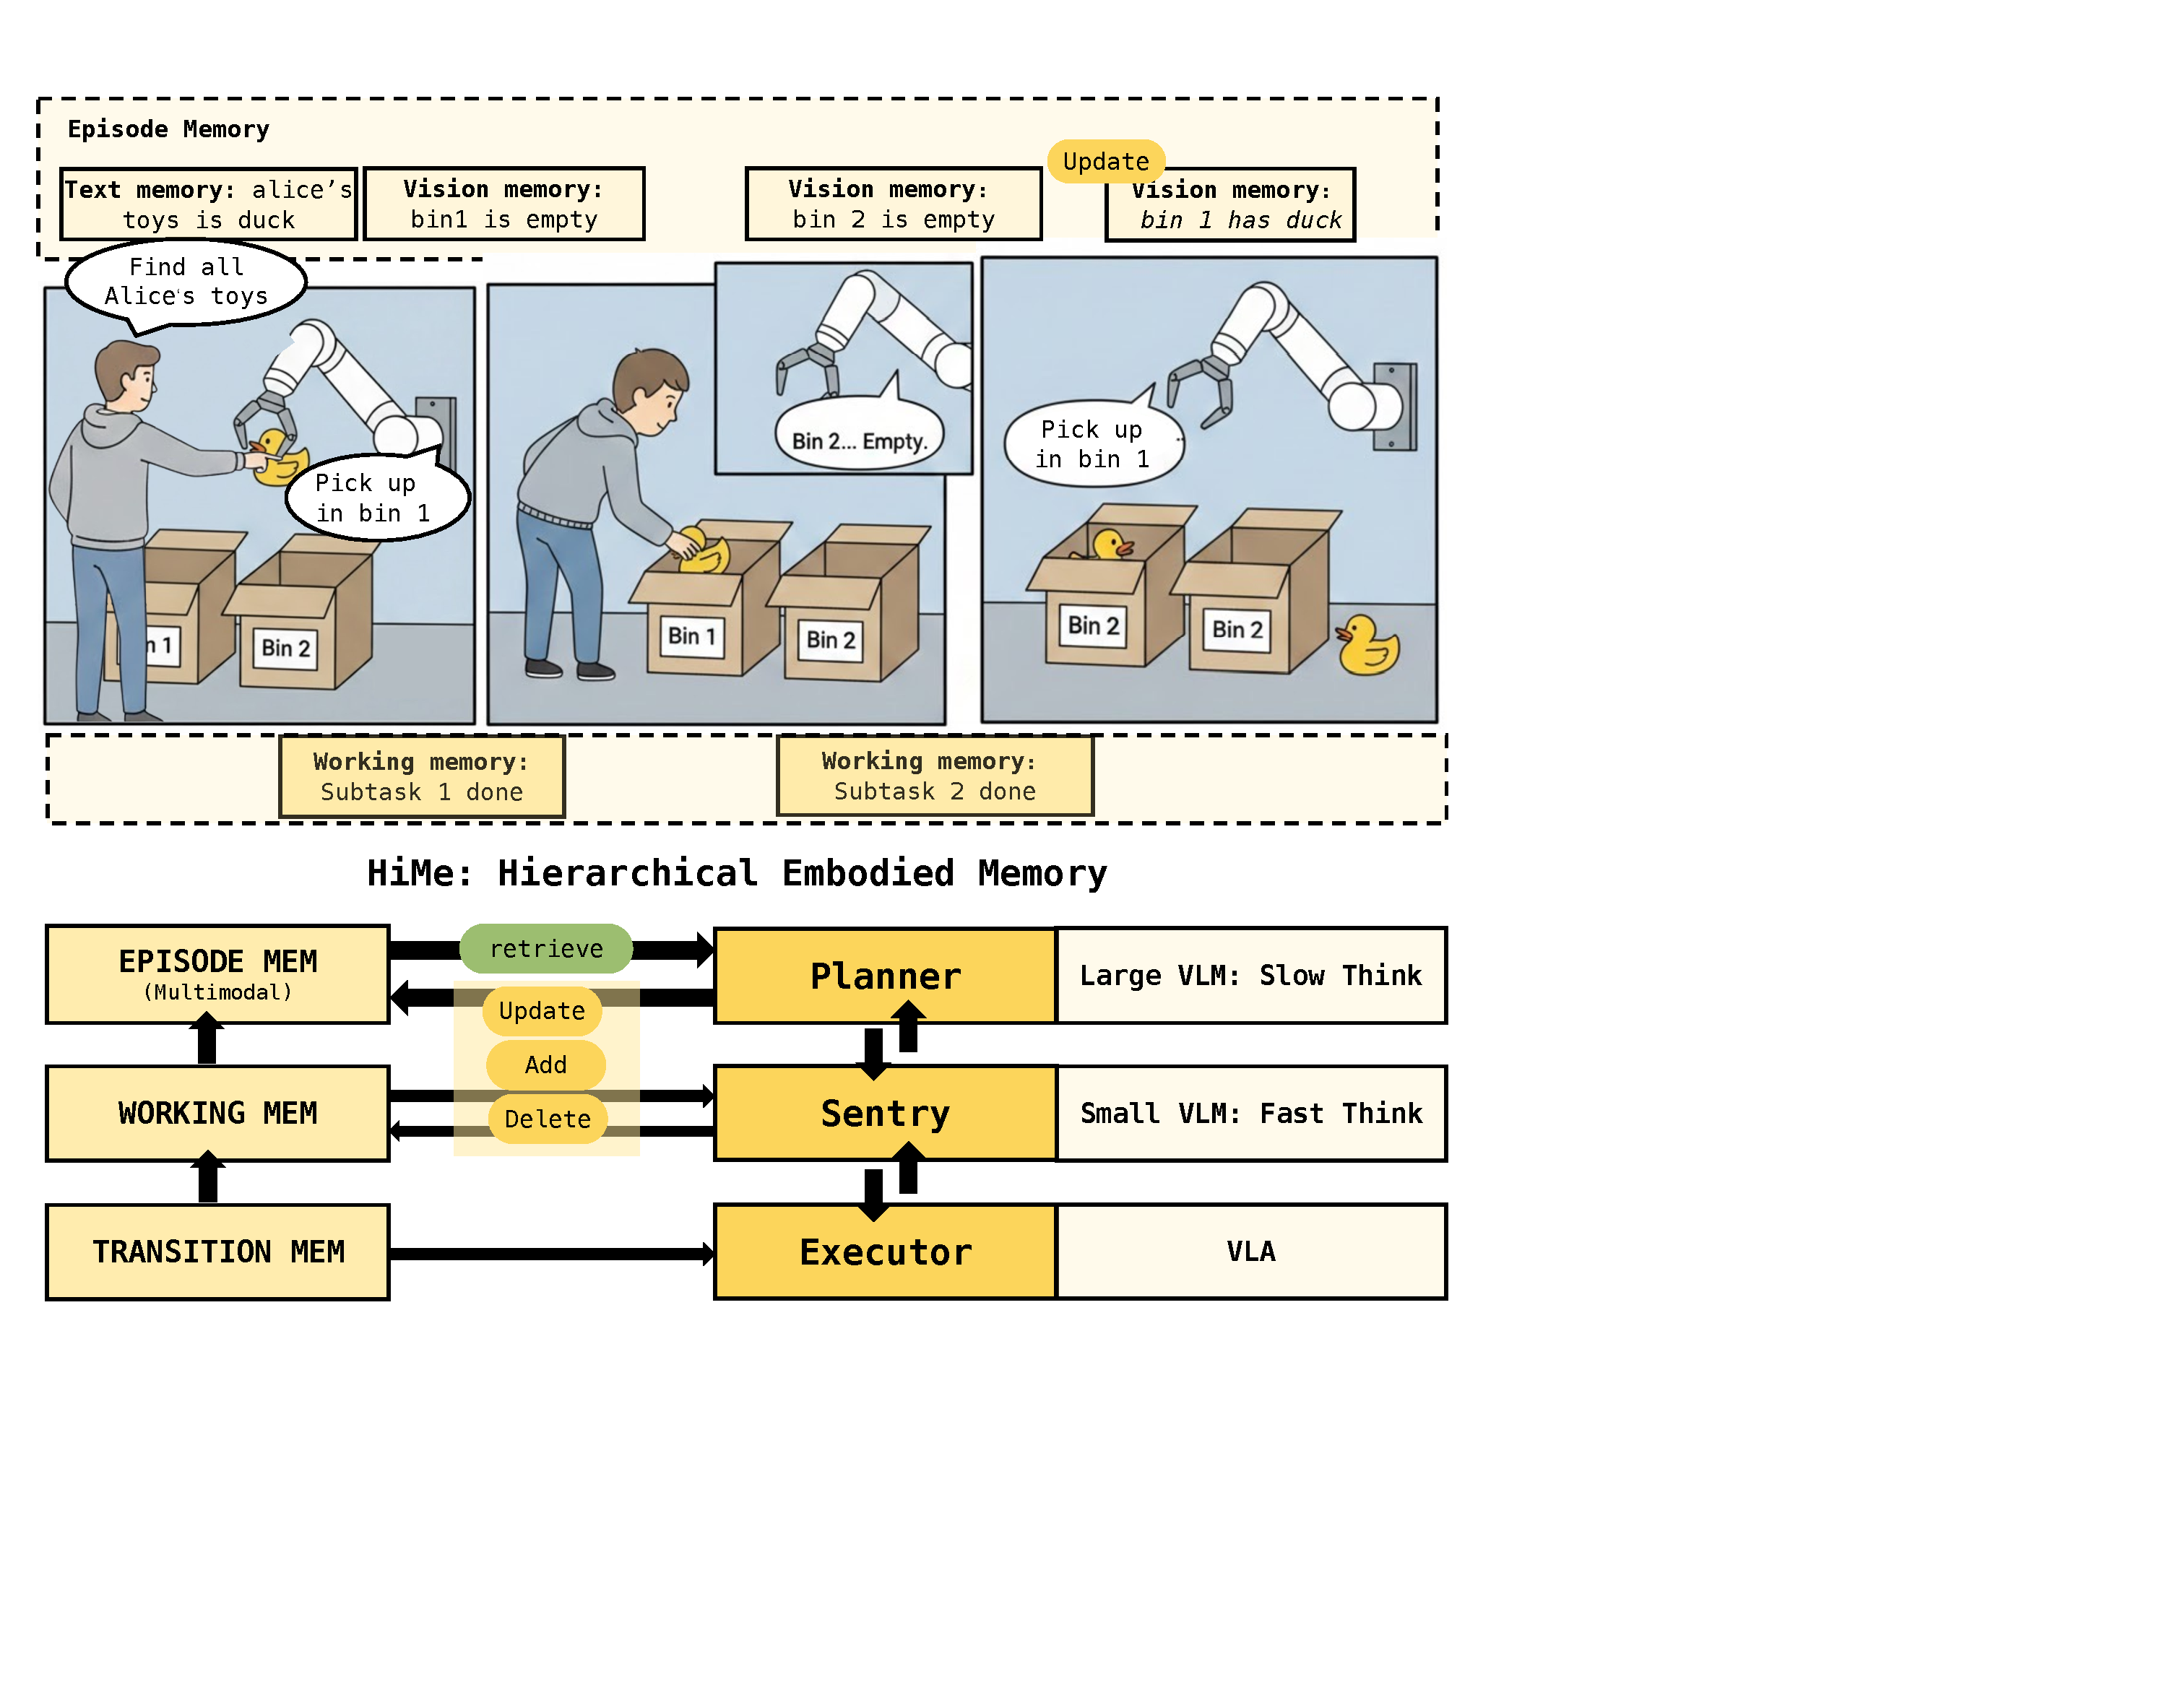
\includegraphics[width=1\linewidth]{imgs/intro.pdf}
    \caption{\textbf{Overview of HiMe.} A motivating example (top) illustrates the need for maintaining and updating task-relevant multimodal memory across long-horizon subtasks. HiMe addresses this challenge by organizing embodied intelligence into a hierarchical structure that separates fast execution from memory-driven reasoning over long time scales. }
    \label{fig:intro}
\end{figure}

% To break the temporal constraints of reactive policies, recent research has explored expanding the observation context. Some approaches utilize auxiliary losses \cite{torne2025} or finetuning to imbue models with native memory capabilities \cite{fang2025}. A notable advancement is MemER \cite{memer2025}, which retrieves historical trajectories and prepends them as visual context for a Vision-Language Model (VLM). However, these methods—including MemER—predominantly adopt a \textbf{flat memory paradigm}. They treat historical data as a static, unmanaged sequence, forcing the model to resolve low-level sensory details and high-level strategic reasoning within the same computational manifold. This leads to an inherent \textbf{granularity conflict}: reactive control demands high-frequency sensory precision, whereas strategic planning requires low-frequency semantic abstraction. Forcing a policy to process an ever-growing, uncurated historical context not only incurs prohibitive computational overhead but also causes the agent to deviate under the distraction of irrelevant sensory noise.

% To overcome these limitations, one intuitive approach is to imbue VLA models with native memory capabilities through specialized training or auxiliary losses \cite{torne2025, fang2025}. However, these training-based methods are often constrained by limited context windows and the inherent difficulty of optimizing long-range causal dependencies over hundreds of steps. Another alternative is to introduce Large Vision-Language Models (VLMs) as high-level memory containers to store and retrieve historical trajectories \cite{memer2025}. Yet, this strategy encounters a fundamental frequency-capability paradox: Utilizing massive, state-of-the-art VLMs for real-time planning introduces prohibitive computational latency that is misaligned with the high-frequency requirements of robotic control. Conversely, opting for smaller, distilled models to reduce latency often requires intensive domain-specific finetuning and inevitably strips the agent of the "slow-thinking" capability—the broad, cross-domain reasoning and zero-shot planning inherent in large-scale models. 

To overcome these limitations, one intuitive approach is to imbue VLA models with native memory capabilities through specialized training or auxiliary losses \cite{Torne2025LearningLD,Fang2025SAM2ActIV}. However, these training-based methods are often constrained by limited context windows and the inherent difficulty of optimizing long-range causal dependencies over hundreds of steps. Another alternative is to introduce Large Vision-Language Models (VLMs) as high-level memory containers to store and retrieve historical trajectories \cite{Sridhar2025MemERSU}. Yet, real-time robotic control imposes a strict upper bound on the deployable VLM scale, as control demands high-frequency, low-latency execution. This scale constraint, in turn, limits the internal world knowledge and generalization capabilities of the VLM, weakening its zero-shot performance. Importantly, most memory operations do not intrinsically require high-level reasoning or broad generalization. 

Motivated by this temporal and scale mismatch, we decouple memory and reasoning operations into hierarchical layers with distinct time scales.
% These observations suggest that the bottleneck of robotic memory is not merely a matter of model scale, but rather an architectural misalignment.
We propose \textbf{HiMe}, a \textbf{Hierarchical Embodied Memory} framework that decouples embodied intelligence into three functional layers with distinct temporal resolutions, mirroring the multi-store structure of human cognition. 
(1) The \textbf{Executor (VLA)} governs \textbf{transient memory}, focusing on high-frequency sensory-motor coordination for physical stability. 
(2) The \textbf{Sentry} acts as the guardian of \textbf{working memory} (short-term memory); it asynchronously filters the continuous sensory stream to identify critical state transitions, effectively bridging the gap between raw perception and semantic events. 
(3) The \textbf{Planner} manages \textbf{episodic memory} (long-term memory). 
By invoking the ``slow-thinking" Planner only at the discrete junctions identified by the Sentry, our architecture preserves deep strategic reasoning while maintaining real-time execution, effectively resolving the frequency-capability paradox.

% Inspired by the multi-store model of human cognition, we propose a \textbf{Hierarchical Memory Management} framework that decouples execution from cognition across three distinct temporal scales. At the base, the \textbf{Executor (VLA)} maintains high-frequency reactive control, modeling \textbf{transient memory} for immediate physical stability. Above this, a \textbf{Monitor} acts as the guardian of \textbf{working memory}; it asynchronously tracks task progress and filters the continuous sensory stream into discrete, task-relevant events. At the apex, a \textbf{Planner} manages \textbf{episodic memory} (long-term experience). The Planner is only invoked at critical junctions identified by the Monitor, allowing it to perform deep reasoning and memory retrieval without interfering with the high-speed execution loop. This hierarchical decoupling ensures that strategic consistency is preserved while maintaining real-time responsiveness.



% However, a static memory hierarchy is insufficient for the complexities of real-world human-robot interaction, which is characterized by \textbf{multimodal richness} and \textbf{high dynamism}. Human instructions often carry dense logical constraints and safety preferences---such as ``this tool is fragile, handle it with care''---which are nearly impossible to capture through vision-only trajectories alone. Furthermore, in open-ended environments, task goals and human preferences are not static; they evolve. A memory system that only supports passive accumulation, such as MemER \cite{memer2025}, inevitably suffers from knowledge stagnation and cognitive dissonance when faced with outdated or conflicting experiences.


However, a static memory hierarchy alone is insufficient for the complexities of real-world human-robot interaction, which is characterized by: (1) \textit{multimodal richness}, where human instructions carry dense logical constraints and latent preferences---such as designating a specific red cup as ``Alice's cup''---that are nearly impossible to capture through vision-only trajectories; and (2) \textit{high dynamism}, where task goals and environment states are not static but evolve. A memory system that only supports passive accumulation~\cite{Sridhar2025MemERSU} inevitably suffers from knowledge stagnation and cognitive dissonance when faced with such outdated or conflicting experiences.

Furthermore, our Hierarchical Memory framework treats memory as a multimodal, dynamic knowledge system centered around two fundamental dimensions:

\textit{(1) What to memorize?: Cross-modal Semantic Schemata.} To bridge the gap between raw perception and logical intent, we represent episodic memory as an object-centric system where visual experiences are deeply anchored with high-density textual descriptions. This organization allows the Planner to retrieve not only visual features but also the underlying ownerships, procedural rules, and human preferences that are invisible in pure pixel space.

\textit{(2) How to memorize?: Active Management Mechanism.} In contrast to passive storage, we introduce explicit \textit{Add}, \textit{Update}, and \textit{Delete} operations to grant the robot knowledge plasticity. When the Sentry detects a significant state transition or a revision in user intent, the Planner proactively refines the knowledge base. By updating outdated beliefs and purging redundant or erroneous data, the agent maintains a consistent and concise memory that evolves in alignment with the environment.



% First, \textit{what should the agent memorize?} To bridge the gap between raw perception and logical intent, we represent episodic memory as \textbf{cross-modal semantic schemata}. Instead of storing raw video frames, we build an object-centric memory bank where visual experiences are deeply anchored with high-density textual descriptions. This organization allows the Planner to retrieve not only visual cues but also the underlying procedural rules and human preferences that are often invisible in pure pixel space. 

% Second, \textit{how should the memory be managed?} In contrast to the passive accumulation seen in prior works \cite{memer2025}, we introduce an \textbf{Active Management Mechanism} consisting of explicit \textit{Add}, \textit{Update}, and \textit{Delete} operations. This grants the robot \textbf{knowledge plasticity}: when the Monitor detects a significant state transition or a deviation in user preference, the Planner proactively refines the knowledge base. By updating outdated beliefs and purging redundant or erroneous experiences, the agent maintains a consistent and concise memory that evolves in alignment with the environment and user intentions.


% In our framework, memory is not merely a passive recording but a \textbf{dynamic, cross-modal knowledge system}. First, we represent episodic memory as semantic schemata, where visual trajectories are deeply anchored with high-density textual descriptions. This organization allows the Planner to bridge the gap between raw perception and logical intent, leveraging human feedback and procedural rules that are often invisible in pure pixel space. Second, we introduce an \textbf{Active Management Mechanism} consisting of explicit \textit{Add}, \textit{Update}, and \textit{Delete} operations. When the Monitor detects a subtask completion or a deviation in human preference, the Planner proactively refines the memory bank. By updating outdated experiences and purging redundant or erroneous data, the agent maintains a consistent and concise knowledge base that evolves alongside the environment and user intentions.

% In this paper, we present \textbf{Active Embodied Memory (AEM)}, a framework that transforms robotic memory from a passive archive into a \textbf{self-evolving knowledge base}. Our contribution is twofold: 
% (1) \textbf{Cross-modal Memory Organization}: We represent experiences as semantic schemata where visual trajectories are deeply anchored with high-density textual descriptions, bridging the gap between raw perception and logical intent. 
% (2) \textbf{Active Management Mechanism}: We introduce explicit \textit{Add}, \textit{Update}, and \textit{Delete} operations, granting the agent \textbf{knowledge plasticity}. By actively refining its memory bank based on real-time interactive feedback, AEM ensures that the robot’s internal knowledge remains consistent, concise, and aligned with evolving human intentions. Our experiments demonstrate that AEM significantly improves success rates in dynamic, long-range tasks, establishing a new paradigm for lifelong embodied learning.

We evaluate our method across a suite of challenging long-horizon manipulation tasks that require multi-step reasoning and adaptation to shifting human preferences. Experimental results show that our approach significantly outperforms existing flat-memory baselines in both success rate and computational efficiency. Notably, our agent demonstrates the ability to ``self-correct" its internal knowledge base when faced with conflicting instructions, a capability that is absent in prior retrieval-based methods.

Our core contributions are summarized as follows:
\begin{itemize} 
    \item We propose a \textbf{Hierarchical Memory Management framework} that decouples robotic control into transient (Executor), working (Sentry), and episodic (Planner) memory layers, resolving the granularity conflict in long-horizon VLA tasks.
    \item  We introduce a Cross-modal Memory organization (\textit{what to memorize}) combined with an Active Management mechanism (\textit{how to memorize}), enabling the robot to maintain knowledge plasticity and alignment in highly dynamic and multimodal interactions.
    \item We provide \textbf{extensive empirical evidence} demonstrating that our hierarchical, self-evolving memory architecture achieves superior performance and robustness in complex human-robot collaborative scenarios with significantly reduced VLM computational overhead.
\end{itemize}

\section{Related Work}

\subsection{Foundation models in robotics}
Recent advancements in End-to-End Vision-Language-Action (VLA) models adopt a co-training paradigm that integrates a pre-trained VLM backbone with a dedicated action expert~\cite{Black20240AV, Intelligence202505AV}. By harnessing the VLM's extensive world knowledge~\cite{Bai2025Qwen3VLTR} to interpret complex scenes, this approach effectively transforms the backbone into a generalist agent capable of mapping raw observations directly to continuous actions. 
Alternatively, the hierarchical paradigm decouples reasoning from execution~\cite{Shi2025HiRO, Li2025HAMSTERHA, Shentu2024FromLT}. In this framework, a high-level policy, typically a VLM, processes visual observations and task descriptions to generate intermediate goals, such as natural language sub-tasks or latent embeddings. These intermediate representations then condition a low-level policy to output continuous actions. Building upon this hierarchical structure, our work introduces a novel hierarchical memory architecture designed to empower the high-level VLM to generate more precise and context-aware instructions for the low-level controller.

% \subsection{Robotic memory}
% Memory capabilities are fundamental for VLA to successfully execute complex, long-horizon manipulation tasks. 
% Consequently, extensive research has been dedicated to endowing vla with historical context, though most existing implementations remain predominantly image-based~\cite{Huang2022VisualLM}. 
% These works typically follow two paradigms: utilizing external memory banks~\cite{Li2025MAPVLAMP, Torne2025LearningLD, Fang2025SAM2ActIV, Huang2023OutOS, Zhu2020VisionDialogNB, Zheng2024TraceVLAVT, Hu20253DLLMMemLS}, that employ FIFO queues~\cite{Sridhar2025MemERSU} or fused buffers~\cite{Shi2025MemoryVLAPM} to store raw observations, or exploring history compression to distill information into compact representations. Notably, MemER~\cite{Sridhar2025MemERSU} recently advanced the latter by proposing keyframe selection algorithms to better preserve critical information within subtasks.
% Distinct from these methods, we propose a cross-modal, explicitly managed memory bank designed to enhance task consistency and effectively retain long-term temporal context.

\subsection{Robotic memory}
Memory is important for robotic agents operating in long-horizon, partially observed manipulation tasks, where successful execution often depends on retaining past observations, inferred world states, and user-specific context. Prior work has therefore explored a range of mechanisms for incorporating historical information into robotic control.

One major direction introduces memory at the policy level, where historical context is used primarily to improve local action generation, spatial grounding, and short-range temporal consistency. Typical approaches either augment Vision-Language-Action models with retrieval-style memory banks that store and retrieve relevant past context~\cite{Li2025MAPVLAMP, Fang2025SAM2ActIV, Zhu2020VisionDialogNB, Shi2025MemoryVLAPM}, or encode history into more compact forms, such as past tokens or visual traces, for history-conditioned action prediction~\cite{Torne2025LearningLD, Zheng2024TraceVLAVT}. 

Another direction studies memory in more structured, higher-level decision processes. Previous hierarchical embodied-agent systems~\cite{Wang2023JARVIS1OM, Li2024Optimus1HM, Wang2023DescribeEP} have highlighted the value of explicit planning, reflection, and multimodal memory for long-horizon decision making. MemER~\cite{Sridhar2025MemERSU} organizes experience through a FIFO queue together with keyframe selection. These works suggest that memory is useful not only for short-range control, but also for maintaining task-level context over extended horizons.

Our work follows this latter direction, and focuses on a multimodal memory design with explicit memory management.
\section{Methods}

\input{030-method-v2}
\section{Experiments}


\subsection{Task Setting}



To demonstrate the critical role of hierarchical memory in long-horizon tasks, we designed three distinct tabletop manipulation scenarios, as illustrated in~\autoref{fig:exp}. These tasks are specifically curated to evaluate diverse capabilities, including user interaction, preference memory, updating memory and planning with exploration.

\textbf{Object Search.} 
We design a Domestic Maintenance task to evaluate the robot's capability to integrate inspection, sorting, and preference recall. In this scenario, the robot must first inspect opaque boxes to deduce storage rules and organize scattered items accordingly. Crucially, during this process, the user introduces new toys into the boxes to test the robot's ability to dynamically update its memory. Finally, the robot faces a retrieval challenge, where it must synthesize memorized user preferences with the box contents identified during inspection to retrieve the correct object.
% \textit{Evaluation metrics.} We evaluate the robot's proficiency by monitoring whether it performs necessary inspections, correctly memorizes box contents, places items in the appropriate containers, updates the memory with the latest observation and successfully retrieves the target object. 

\textbf{Counting.} 
In this scenario, the robot is required to interpret a visual recipe on the table and plan its subsequent actions. The task proceeds in stages: the robot must first \textit{inspect} the recipe to extract the ingredient composition and prepare the materials based on the number of servings requested by the user. Following this, the user introduces a specific preference. To fulfill this customized demand, the robot must synthesize the new constraint with the previously memorized recipe to dispense the correct personalized ingredients.
% \textit{Evaluation metrics.} We assess the robot's performance based on three criteria: (1) whether the robot actively and correctly inspected the visual recipe; (2) the accuracy of the ingredient preparation relative to the recipe and requested servings; and (3) whether the robot succeed in satisfying the final customized user preference.

\textbf{Rearrangement.} 
In this playroom scenario, the robot performs a two-stage ``clear and restore'' operation. Initially, the robot collects all toys scattered on the table into a storage box for cleaning. After a temporal interval, the robot is tasked with restoring the items to the environment. Crucially, the user's specific placement preference is provided beforehand as prior knowledge. Therefore, to execute the restoration, the robot must recall this pre-established preference and synthesize it with its visual memory of the original spatial configuration to plan the final placement of each item.
% \textit{Evaluation metric.} We measure task success based on two criteria: (1) the completeness of the initial collection into the storage box; and (2) the accuracy of the final restoration, specifically whether items were placed in the correct location.

\textbf{Evaluation Setup}
We use a WidowX-250s arm with a parallel gripper and dual-camera visual input (third-person and wrist view). The Executor $\pi_e$ runs at 2\,Hz, predicting an action chunk $A_t$ of 10 actions (10\,Hz), of which 5 are executed open-loop. To monitor the subtask progress, the Sentry $\pi_s$ is queried after every 10 execution steps of $\pi_e$. The Sentry will trigger Planner $\pi_p$ if the current subtask is completed for slow thinking.
Each task’s evaluation metrics are detailed in \autoref{app:eval}.




\subsection{Main Experiment}

% no memory: 只有 subtask， 1帧 GPT-4o+VLA (去掉planner和monitor）
% no memory + monitor： 只有 subtask， 8帧给 monitor 1帧给GPT-4o （去掉planner的memory能力）
% memer: planner只输出subtask， 超过 距离 8 则filter关键帧； 看临近8帧
% ours
% human 
% \paragraph{Main experiment.}

To thoroughly validate the effectiveness of our \emph{hierarchical memory} and the \emph{monitor-based} trigger mechanism, we keep the low-level policy $\pi_{\text{l}}$ and the planner backbone constant, varying only the \textbf{memory context} and the \textbf{planning frequency}. The comparisons are designed as follows:

% \siyin{add a table to compare all the methods: sentry/frequency(fix-interval vs trigger), memory (no, keyframe context, database)}
% (Place after "The comparisons are designed as follows:" or right before the itemize.)

% \begin{itemize} [itemsep=0.1em, topsep=0.3em]
%     \item \textbf{Transient Memory:} 
%     A standard hierarchical VLA baseline where a memory-less planner is invoked at fixed intervals ($n_m$) and observes only the current frame $o_t$. This represents the current paradigm of hierarchical robot foundation models, such as Hi-robot~\cite{Shi2025HiRO}.
%     % We remove the monitor module and the memory database. The planner $\pi_{\text{high}}$ is invoked at a fixed frequency and receives only the current frame $o_t$. This serves as a reactive baseline similar to standard hierachy VLA setups without temporal aggregation.
    
%     \item \textbf{Transient Memory w/ Sentry:} 
%     This variant introduces our Sentry module to trigger the planner based on task progress. However, the planner remains memory-less, receiving only $o_t$ upon being triggered. It evaluates the benefit of the more stablized planning from the sentry's gating.
%     % We introduce the monitor, providing it with the most recent 8 frames to decide whether the current subtask has terminated. However, when the planner is triggered, it still receives only the latest frame $o_t$ to predict the next subtask. This baseline isolates the benefit of the \emph{monitor's timing} from the \emph{planner's memory}.
    
%     \item \textbf{Flat Memory:} 
%     The planner operates at a fixed frequency and receives the 8 most recent observations, assisted by a FIFO queue of historical keyframes it previously selected. This setting tests whether unstructured, flat memory is sufficient for long-horizon tasks. This setting is similar to MemER \cite{Sridhar2025MemERSU}.
%     % To compare our hierarchical structure against flat retrieval methods, we implement a baseline inspired by MemER. The planner operates at a fixed frequency (without a monitor) and receives a context consisting of the recent 8 frames plus a FIFO queue of keyframes from the history. This tests whether unstructured keyframe retention is sufficient for long-horizon consistency.
    
%     \item \textbf{HiMe w/o Sentry:} 
%     We utilize our complete planner's memory design but remove the sentry module. The planner is forced to query the VLM at a fixed frequency regardless of subtask progress. This ablation validates the sentry's role in reducing computational redundancy and aligning planning steps with the dyanmics of environments.
    
%     \item \textbf{HiMe (Ours):} 
%     The proposed framework, where the monitor dynamically triggers planning based on subtask progress, and the planner utilizes the full hierarchical memory to ensure global consistency.
    
%     \item \textbf{Human High-level:} 
%     A human oracle provides the correct subtask description at each step. This serves as an upper bound on task performance given the fixed capabilities of $\pi_{\text{l}}$.

% \end{itemize}

\textbf{Transient Memory:} 
    A standard hierarchical VLA baseline where a memory-less planner is invoked at fixed intervals ($n_m$) and observes only the current frame $o_t$. This represents the current paradigm of hierarchical robot foundation models, such as Hi-robot~\cite{Shi2025HiRO}.
    % We remove the monitor module and the memory database. The planner $\pi_{\text{high}}$ is invoked at a fixed frequency and receives only the current frame $o_t$. This serves as a reactive baseline similar to standard hierachy VLA setups without temporal aggregation.
    
\textbf{Transient Memory w/ Sentry:} 
    This variant introduces our Sentry module to trigger the planner based on task progress. However, the planner remains memory-less, receiving only $o_t$ upon being triggered. It evaluates the benefit of the more stablized planning from the sentry's gating.
    % We introduce the monitor, providing it with the most recent 8 frames to decide whether the current subtask has terminated. However, when the planner is triggered, it still receives only the latest frame $o_t$ to predict the next subtask. This baseline isolates the benefit of the \emph{monitor's timing} from the \emph{planner's memory}.
    
\textbf{Flat Memory:} 
    The planner operates at a fixed frequency and receives the 8 most recent observations, assisted by a FIFO queue of historical keyframes it previously selected. This setting tests whether unstructured, flat memory is sufficient for long-horizon tasks. This setting is similar to MemER \cite{Sridhar2025MemERSU}.
    % To compare our hierarchical structure against flat retrieval methods, we implement a baseline inspired by MemER. The planner operates at a fixed frequency (without a monitor) and receives a context consisting of the recent 8 frames plus a FIFO queue of keyframes from the history. This tests whether unstructured keyframe retention is sufficient for long-horizon consistency.
    
\textbf{HiMe w/o Sentry:} 
    We utilize our complete planner's memory design but remove the sentry module. The planner is forced to query the VLM at a fixed frequency regardless of subtask progress. This ablation validates the sentry's role in reducing computational redundancy and aligning planning steps with the dyanmics of environments.
    
\textbf{HiMe (Ours):} 
    The proposed framework, where the Sentry dynamically triggers planning based on subtask progress, and the planner utilizes the full hierarchical memory to ensure global consistency.
    
\textbf{Human High-level:} 
    A human oracle provides the correct subtask description at each step. This serves as an upper bound on task performance given the fixed capabilities of $\pi_{l}$.


%  ===== Experiment Setting's Table =====
\newcommand{\TabW}{\dimexpr\columnwidth-6\tabcolsep\relax}

\begin{table}[t]
    \centering
    \small
    \setlength{\tabcolsep}{2.5pt}
    \renewcommand{\arraystretch}{1.12}
    % TODO: Adjust column width after content finalization
    \caption{
    Comparison of hierarchical settings in the main experiment. }
    \label{tab:main_settings}

    \begin{tabular}{@{}
    p{0.475\TabW}
    p{0.175\TabW}
    p{0.35\TabW}
    @{}}
        \toprule
        \textbf{Hierarchy Setting} & \textbf{Trigger} & \textbf{Planner Memory} \\
        \midrule
        Transient Memory
            & Periodic
            & Current observation \\
        Transient Memory w/ Sentry
            & Sentry
            & Current observation \\
        Flat Memory
            & Periodic
            & Recents + FIFO \\
        HiMe w/o Sentry
            & Periodic
            & Recents + keyframes \\
        HiMe (Ours)
            & Sentry
            & Recents + keyframes \\
        Human High-level
            & Sentry
            & Human oracle \\
        \bottomrule
    \end{tabular}
    \vspace{-0.6em}
\end{table}

% To validate the effectiveness of our proposed \emph{hierarchical memory} design, we keep the same low-level policy $\pi_{\text{low}}$ and high-level policy backbone $\pi_{\text{high}}$ across all settings, and \emph{only} vary the memory structure of $\pi_{\text{high}}$ (i.e., what context it observes and how it is invoked). This isolates the contribution of hierarchical memory from other confounding factors. We compare against the following baselines. 
% \emph{No memory}: we remove the monitor module and provide $\pi_{\text{high}}$ only the current frame at each planning step, requiring it to predict the subtask to execute next. 
% \emph{No memory w/ monitor}: we provide the monitor with the most recent 8 frames to decide whether the current subtask has terminated; however, each time the planner calls $\pi_{\text{high}}$, it still receives only the latest frame and must predict the next subtask. 
% \emph{Short memory + monitor}: building on \emph{No memory}, each planner call provides $\pi_{\text{high}}$ with 8 frames uniformly sampled from the execution history of the current subtask, and asks it to predict the next subtask. 
% \emph{MemER} 
% \emph{Ours}: a complete hierarchical memory design, 
% \emph{planner memory} similar to MemER
% Finally, we design a keyframe filter

% \emph{Human high-level}: a human oracle provides the correct subtask at each step, which serves as an upper bound on task performance given the fixed $\pi_{\text{low}}$.

% 这个主实验应该就是用来说明层次化记忆的用处
% 1. no memory VS no memory+monitor --》用来说明monitor的控制很重要(monitor拆解subtask，调节 planner的控制频率和vla的动作频率）
% 2. no memory+monitor VS  ours --》用来说明long-term memory的重要
% 3. no memory VS MemER vs Ours --> memer通过关键帧的筛选解决了一部分问题，但如果大模型做planner也会出现 仍然存在xx （


% \subsection{Q1: How much does the Sentry mechanism contribute to the overall performance?}
\subsection{Analysis of Sentry Mechanism}
\label{sec:sentry}
We analyze the Sentry mechanism's contribution from two key dimensions: \textit{execution consistency} and \textit{observation quality}.

\textit{1) Consistency via Reduced Task Switching:}
Even in a Planner with transient memory setting, the Sentry significantly boosts performance. 
In \autoref{fig:main}, we observe a substantial improvement ($14\%$ vs. $26\%$) when comparing \textit{Transient Memory} with \textit{Transient Memory w/ Sentry}. Without the Sentry, the planner operates on a frame-by-frame style, and this high-frequency re-evaluation makes the robot hypersensitive to transient visual noise, leading to frequent, erratic switching between subtasks. The Sentry prevent the planner from intervening until the current subtask is completed, reducing unnecessary task switching and ensures that actions are executed coherently. It reveals that \textbf{the core value of the Sentry here is enforcing temporal consistency of Planner.}

% Comparing \textit{Transient Memory} with \textit{Transient Memory w/ Sentry} (\autoref{fig:main}), we observe a substantial improvement ($14\%$ vs. $26\%$).
% \textbf{The core value of the Sentry here is enforcing temporal consistency.}
% Without the Sentry, the planner operates on a frame-by-frame basis. This high-frequency re-evaluation makes the agent hypersensitive to transient visual noise, leading to frequent, erratic switching between subtasks. The Sentry acts as a temporal lock, preventing the planner from intervening until the current subtask is completed. This reduces unnecessary task switching and ensures that actions are executed coherently.

\textit{2) Quality via Uniform Sampling vs. Recent Frames:}
% \siyin{experiment results --> conclusion.}
% Beyond consistency, the Sentry improves the quality of information provided to the planner.
% While a standard planner only sees a narrow window of recent frames, the Sentry accumulates the entire history of the executed subtask and provides a uniformly sampled overview.
% This is crucial for verifying success. A planner looking only at the last few frames might miss the context of the action, whereas the Sentry's global view allows the planner to verify the entire progression of the subtask, further reducing hallucination and replanning.

% Beyond consistency, the Sentry module significantly improves the quality of information provided to the planner, a benefit directly reflected in the substantial performance gap between \textbf{ours-sentry} and ours (\textbf{HiMe}).
% While the ablation model is constrained to a narrow window of recent frames, the Sentry accumulates the entire history of the executed subtask to provide a uniformly sampled overview.
% This global perspective is crucial for verifying success; for instance, a planner relying solely on recent observations might miss the context of an action, whereas the Sentry enables the verification of the entire subtask progression.
% Consequently, this capability to validate long-term execution effectively reduces hallucination and replanning, driving the average task progress from 68\% in \textbf{ours-sentry} to 90\% in \textbf{HiMe}.
% The Sentry's ability to consolidate raw observations into high-quality working memory is a primary factor in the performance gap between the \textit{HiMe w/o Sentry} and \textit{HiMe}, with average task progress increasing from $68\%$ to $90\%$. While standard planners are constrained to a narrow window of recent frames, the Sentry accumulates the entire history of the active subtask to form a structured working memory. By providing a uniformly sampled overview rather than transient snapshots, it offers a global perspective crucial for success verification. For instance, while recent frames may miss the full context of a physical interaction (e.g., the complete trajectory of a push), this consolidated working memory allows the Planner to verify the entire progression, effectively reducing hallucinations and redundant replanning.

The Sentry's ability to consolidate observations into high-quality working memory largely explains the gap between \textit{HiMe w/o Sentry} and \textit{HiMe}, with average task progress rising from $68\%$ to $90\%$. Whereas standard planners rely on a narrow window of recent frames, Sentry aggregates the history of the active subtask into structured working memory. This provides a global perspective for success verification, and the consolidated memory allows the Planner to verify the entire progression, effectively reducing hallucinations and redundant replanning.

\begin{figure*}
    \centering
    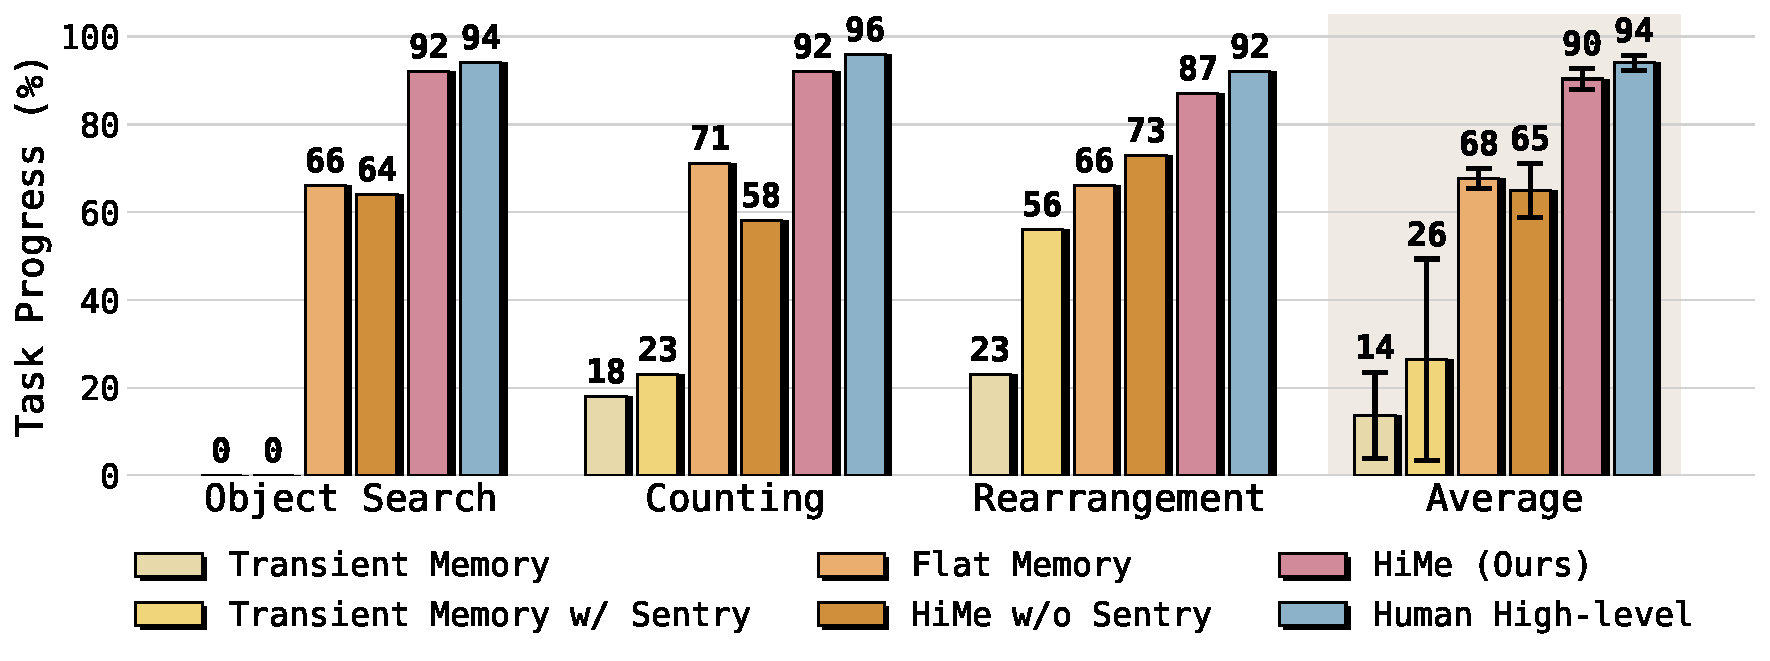
\includegraphics[width=0.98\linewidth]{imgs/6bars.pdf}
    \caption{\textbf{Main Results.} We compare HiMe against Transient, Sentry, and Flat Memory baselines across three long-horizon tasks. HiMe significantly outperforms all baselines, achieving a 90\% average success rate. Notably, our method effectively bridges the gap between robot and the Human High-level oracle.}
    \label{fig:main}
\end{figure*}


% \subsection{Q2: Effectiveness of Hierarchical Memory Architecture}
% \subsection{Q2: How does the Planner's episode memory management contribute to overall performance?}
\subsection{Analysis of Planner Memory Management}
\label{sec:memory}
We validate the necessity of our hierarchical design by comparing \textit{HiMe} against memory-free baselines and flat contextual memory approaches.

\textit{(1) The Necessity of Memory:}
% Long-horizon tasks impose strict requirements on state tracking. In the \textit{Counting} task, even with the Sentry's stability (\textit{No mem + sentry}), the agent fails ($23\%$) because it lacks persistence. Without an explicit memory module, the agent cannot retain states (e.g., counted objects) once they leave the immediate context window.
Long-horizon tasks require persistent state tracking. In \textit{Counting}, even with Sentry stabilization (\textit{Transient Memory w/ sentry}), the robot still fails ($23\%$) due to the lack of persistence: without an explicit memory management, it cannot retain states (e.g., counted objects) once they leave the transient observable state.

\textit{(2) Consolidation vs. FIFO Queues:}
A critical insight from \autoref{fig:main} is the inefficiency of \textit{Flat Memory}, which functions as a contextual memory based on FIFO queues. Although it stores history, it achieves a significantly lower task progress ($65\%$) compared to \textit{HiMe} ($90\%$).
The fundamental limitation of such contextual memory is the lack of consolidation: a simple FIFO queue cannot distinguish between truly critical frames and redundant observations.
In long-horizon tasks, the limited context window is quickly flooded with noisy frames, causing earlier critical information to be discarded. \textit{HiMe} addresses this by actively consolidating memory at the subtask level. This ensures that essential high-level information is preserved regardless of the episode length, enabling high-precision retrieval with minimal planner overhead. 



% \paragraph{Memory modality.}
% Robotic tasks impose heterogeneous memory requirements: the agent must retain \emph{visual} evidence (e.g., object locations and spatial relationships) while also tracking \emph{symbolic} and longitudinal information (e.g., user preferences, task progress, and constraints). Accordingly, we adopt a \textbf{hybrid image--text memory} as the default design, where each memory item can include both an image and a textual description. To assess whether multi-modal storage is necessary, we compare against two unimodal baselines. \emph{Image-only memory} restricts each entry to $(\text{tag}, \text{image}, \text{caption})$, where $\text{tag}$ and $\text{caption}$ are used only for indexing and retrieval, but the response to a query returns only the image. \emph{Text-only memory} restricts each entry to $(\text{tag}, \text{content})$ and enforces that $\text{content}$ is strictly textual (i.e., no images or visual representations).



\section{Further Analysis}

\subsection{Q1: What Type of Memory Representation is Most Effective for Robotic Tasks?}
We investigate the impact of memory modality by comparing purely text memory (\textit{Only text}), purely visual memory (\textit{Only image}), and our cross-modal approach. 

\textit{1) Spatial and Recognition Demands in Robotics:}
% Although many agentic memory systems opt for purely textual captions to minimize storage, our results suggest this is insufficient for physical interaction. Robotic tasks fundamentally rely on spatial relations, object localization, and precise recognition—information where visual data naturally excels.
% Relying solely on text becomes catastrophic when the initial perception model fails to fully recognize an object or accurately describe its spatial context. Text is a form of lossy compression; once the raw visual data is discarded, the robot loses the ability to perform visual re-grounding to recover these spatial details or correct initial recognition errors. In \textit{Object Search}, \textit{Only image} ($86\%$) significantly outperforms \textit{Only text} ($74\%$) for this reason.
Our study results show that robotics tasks impose strong spatial localization and fine-grained recognition demands that caption only memory is inadequate for dynamical physical interactions. Text is a lossy compression: if perception initially misses an object or its spatial context, discarding raw visuals prevents visual re-grounding to recover details or correct errors. In \textit{Object Search}, \textit{Only image} ($86\%$) substantially outperforms \textit{Only text} ($74\%$), which shows that memory with visual evidences is significantly stronger. 


\textit{2) Text for Semantics and Logic:}
% Conversely, text memory is indispensable for non-spatial reasoning. It is far more efficient for summarizing semantic information, analyzing logical dependencies (e.g., task sequencing), and retaining user preferences.
% In tasks requiring abstract reasoning like \textit{Counting}, \textit{Only text} ($91\%$) dominates \textit{Only image} ($78\%$), as these symbolic rules are difficult to extract from pixels on demand.
Conversely, text memory is indispensable for non-spatial reasoning. It efficiently summarizes semantics, captures logical dependencies like task sequencing, and retains user preferences. 
In tasks requiring semantic reasoning, such as \textit{Counting}, \textit{Only text} ($91\%$) outperforms \textit{Only image} ($78\%$), since these semantic clues are hard to extract from pixels on demand.


\textit{3) Superiority of Interleaved Memory:}
% Our cross-modal approach achieves the highest performance (Average $90\%$). By combining the spatial and recognitional fidelity of images with the semantic and logical structure of text, the system ensures the robot can both locate objects precisely in the physical world and reason effectively about user intent.
Our cross-modal approach achieves the best performance (Average $90\%$) by combining the spatial/recognitional fidelity of images with the semantic and logical structure of text, enabling our hierarchical memory system can perform both precise grounding and effective reasoning.



\begin{table*}[t]
\centering
% 使用 resizebox 确保表格适应页面宽度
\caption{Comparison of different methods. We report API calls, memory hit, and average scores across three tasks. Here, API Calls refers to the average Planner requests per subtask, and Memory Hit measures the presence of required information in memory during memory-dependent subtask.}\label{tab:comparison}
\resizebox{\textwidth}{!}{
\begin{tabular}{l ccc ccc ccc ccc}
\toprule
% 第一行表头：大标题
\textbf{Method} & \multicolumn{3}{c}{\textbf{Components}} & \multicolumn{3}{c}{\textbf{Search \& Retrieval}} & \multicolumn{3}{c}{\textbf{Counting}} & \multicolumn{3}{c}{\textbf{Clear \& Restore}} \\
\cmidrule(lr){2-4} \cmidrule(lr){5-7} \cmidrule(lr){8-10} \cmidrule(lr){11-13}

% 第二行表头：具体的列名
% Components 部分
 & \textbf{Sentry} 
 & \textbf{\begin{tabular}[b]{@{}c@{}}Memory\\Management\end{tabular}} 
 & \textbf{\begin{tabular}[b]{@{}c@{}}Memory\\Size\end{tabular}}
% Search & Retrieval 部分
 & \textbf{\begin{tabular}[b]{@{}c@{}}API\\Call ($\downarrow$)\end{tabular}} 
 & \textbf{\begin{tabular}[b]{@{}c@{}}Memory\\Hit ($\uparrow$)\end{tabular}} 
 & \textbf{\begin{tabular}[b]{@{}c@{}}Avg.\\Score ($\uparrow$)\end{tabular}} 
% Counting 部分
 & \textbf{\begin{tabular}[b]{@{}c@{}}API\\Call ($\downarrow$)\end{tabular}} 
 & \textbf{\begin{tabular}[b]{@{}c@{}}Memory\\Hit ($\uparrow$)\end{tabular}} 
 & \textbf{\begin{tabular}[b]{@{}c@{}}Avg.\\Score ($\uparrow$)\end{tabular}} 
% Clear & Restore 部分
 & \textbf{\begin{tabular}[b]{@{}c@{}}API\\Call ($\downarrow$)\end{tabular}} 
 & \textbf{\begin{tabular}[b]{@{}c@{}}Memory\\Hit ($\uparrow$)\end{tabular}} 
 & \textbf{\begin{tabular}[b]{@{}c@{}}Avg.\\Score ($\uparrow$)\end{tabular}} \\
\midrule

HiMe (Ours) & $\checkmark$ & $\checkmark$ & $infinite$ & \textbf{1.8} & \textbf{94\%} & \textbf{92\%} & \textbf{2.6} & \textbf{98\%} & \textbf{92\%} & \textbf{1.4} & \textbf{92\%} & \textbf{87\%} \\
Keyframe Memory & $\times$ & $\times$ & $recent \ 8$ & 5.4 & 68\% & 64\% & 4.8 & 61\% & 58\% & 6.2 & 76\% & 73\% \\
% HiMe w/o Sentry & $\checkmark$ & $\checkmark$ & $\times$ & 20 & 75\% & 0.82 & 15 & 70\% & 0.78 & 28 & 65\% & 0.72 \\
\bottomrule
\end{tabular}
}
\end{table*}
% \subsection{Q2: Are Dynamic Memory Maintenance (Update \& Delete) Necessary?}
\subsection{Q2: Are Dynamic Memory Management Necessary?}

% To validate the necessity of our proposed memory operations, we conducted an ablation study comparing our full method against two baselines: (1) \textit{No Management:} A baseline that only supports \texttt{Add} and \texttt{Retrieve} operations. It retains all historical observations without modification, effectively acting as an append-only buffer. (2) \textit{FIFO:} A variant of \textit{No Management} with a fixed memory capacity (8 entries). When the buffer is full, the earliest entries are evicted to make room for new ones.

To assess the need for dynamic memory management, we run an ablation against two baselines: (1) \textit{No Management}, which only supports \texttt{Add}/\texttt{Retrieve} and keeps all observations as an append-only buffer; and (2) \textit{FIFO}, which caps memory at 8 entries and evicts the oldest when full.

\textit{1) The Cost of Forgetting:}
% As shown in \autoref{fig:manage}, \textit{FIFO} performs the worst ($68\%$ average), significantly lagging behind \textit{No Management} ($86\%$). This performance drop demonstrates that in long-horizon tasks, \textbf{early historical context is crucial}. A fixed-size buffer with naive eviction discards essential information (e.g., the location of an object seen early in the episode) that is required for later reasoning.
In \autoref{fig:manage}, \textit{FIFO} performs worst ($68\%$ average), far below \textit{No Management} ($86\%$). This shows that for long-horizon tasks, \textbf{early context is critical}: naive eviction can remove essential information (e.g., an object location observed early) needed for later reasoning.

\textit{2) The Value of Consistency:}
While \textit{No Management} achieves decent performance by retaining all history, it is still inferior to our full method ($86\%$ vs. $90\%$).
% The limitation of \textit{No Management} lies in \textbf{redundancy and inconsistency}. Without the \textit{Update} and \textit{Delete} operations, the memory accumulates obsolete states (e.g., an object's previous location) alongside current states. This conflicting information introduces noise during the \textit{Query} process, potentially confusing the planner.
Although \textit{No Management} retains all history, it remains below our full method ($86\%$ vs. $90\%$) due to \textbf{redundancy and inconsistency}. Without \textit{Update}/\textit{Delete}, memory stores obsolete states (e.g., prior object locations) alongside current ones, introducing noise during \textit{Query} and potentially confusing the planner.

\textit{3) Necessity of Active Management:}
% Our method achieves the best performance by actively maintaining the memory. The \textit{Update} mechanism ensures state consistency by refreshing outdated entries, while \textit{Delete} removes redundancy. This proves that simply storing more data is not enough; the robot must actively curate its memory to maintain a concise and consistent memory.
Our method performs best by actively curating memory: \textit{Update} refreshes outdated entries to maintain consistency, and \textit{Delete} removes redundancy. Thus, storing more data is insufficient; effective robots must maintain a concise, consistent memory.



\begin{figure}
    \centering
    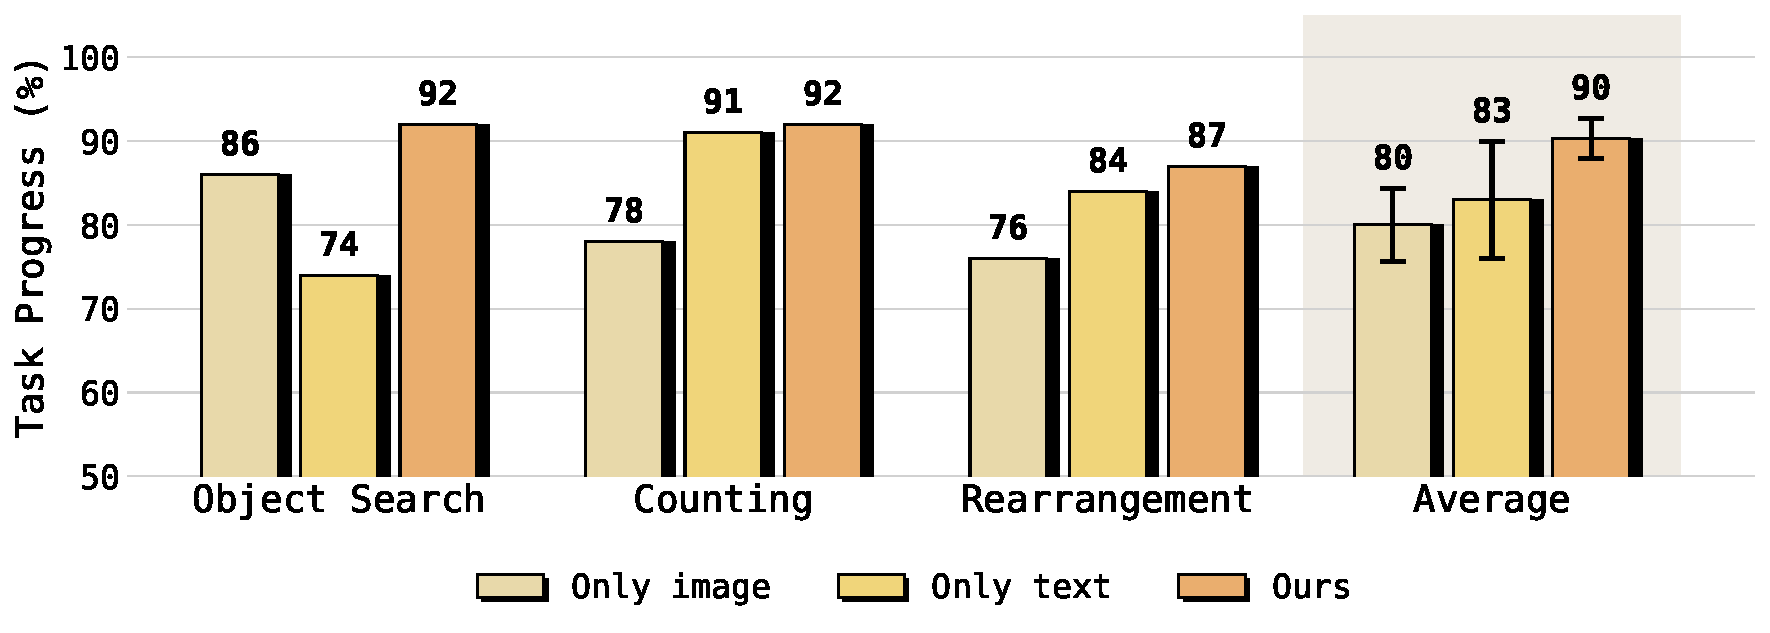
\includegraphics[width=1\linewidth]{imgs/modality.pdf}
    \caption{\textbf{Ablation of Modality.} HiMe consistently outperforms both text-only and image-only baselines across all three tasks, verifying the robustness of our cross-modal memory mechanism.}
    \label{fig:modality}
\end{figure}

% \paragraph{Memory management.}
% Beyond modality, we study whether explicit memory management improves robotic task performance. An effective memory system should remain accurate and up-to-date, reducing the impact of hallucination-induced erroneous entries and reflecting the current world state as the task progresses. We therefore compare our full method (supporting \emph{add/query/update/delete}) against two management baselines that only allow \emph{add} and \emph{query}: (i) \emph{No management}, which disables updates and deletions entirely while keeping all other settings fixed; and (ii) \emph{FIFO}, which maintains a fixed-capacity buffer of size $n$ (set to the average memory size observed under \emph{No management}) and evicts the oldest entries when full, mimicking a standard bounded replay buffer.


\begin{figure}
    \centering
    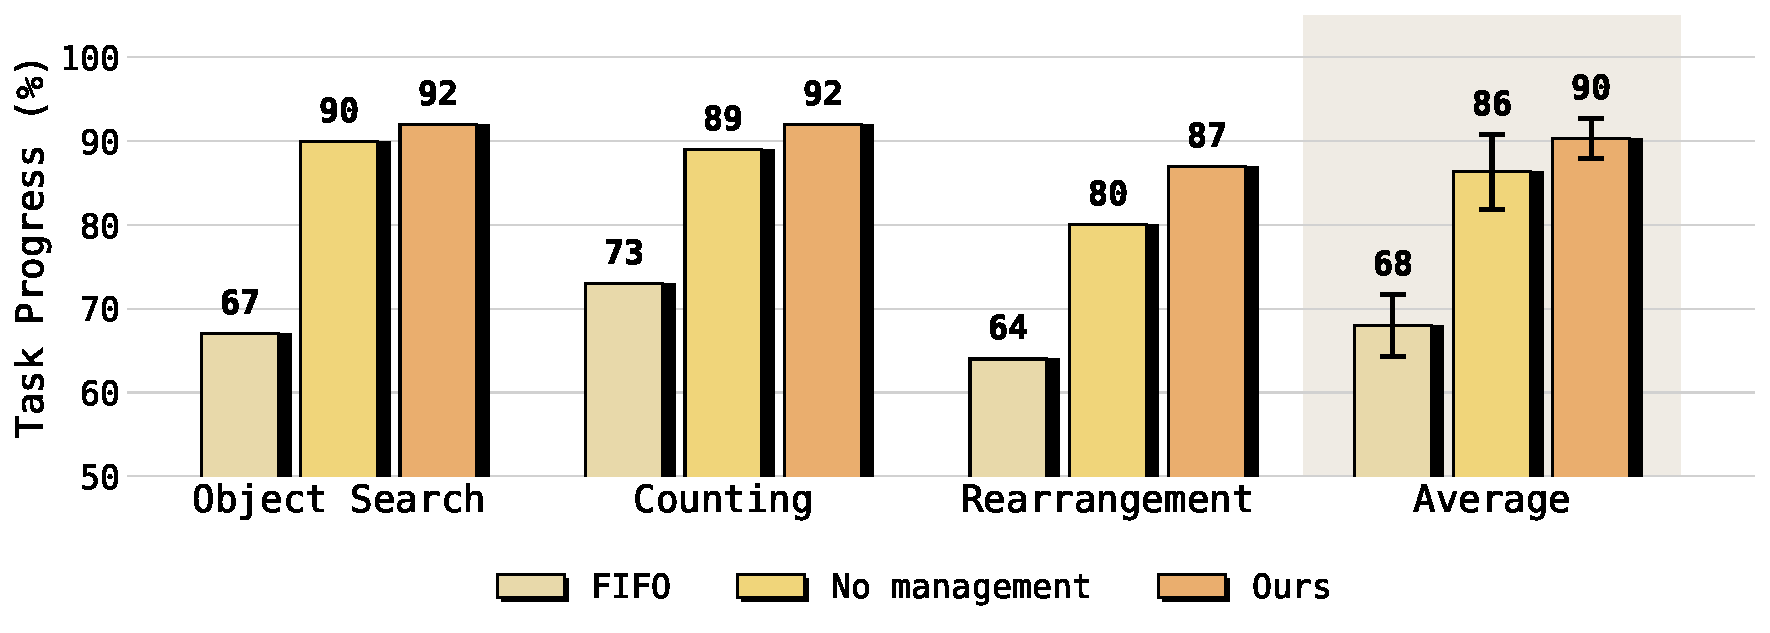
\includegraphics[width=1\linewidth]{imgs/management.pdf}
    \caption{\textbf{Ablation of Management.} Comparison between FIFO, No management, and our approach. HiMe consistently achieves the highest task progress across all three tasks, proving the effectiveness of our memory retrieval and consolidation mechanism in long-horizon tasks.}
    \label{fig:manage}
 \end{figure}

% \begin{figure}
%     \centering
%     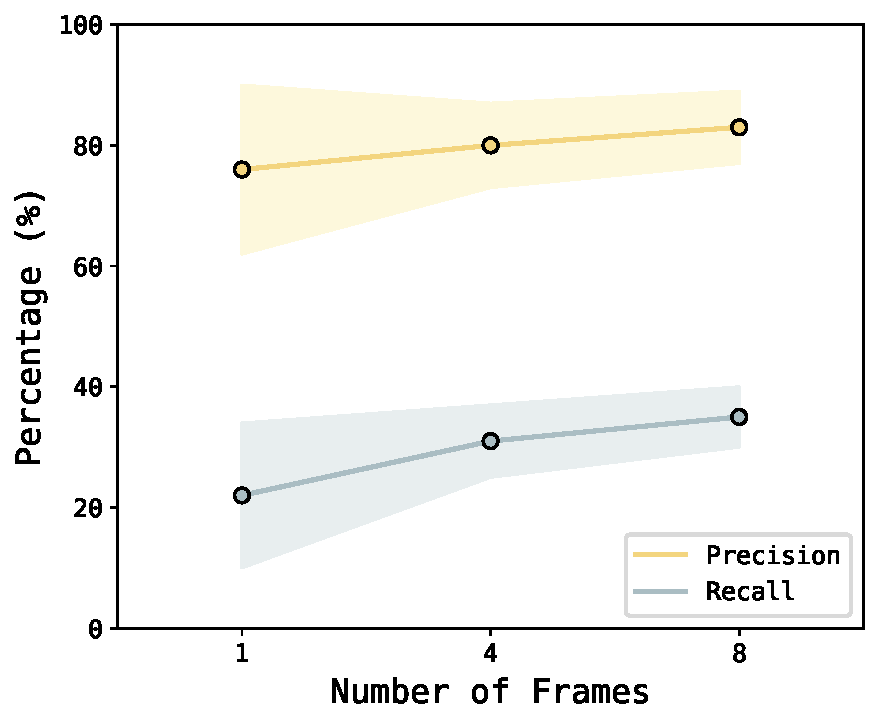
\includegraphics[width=1\linewidth]{imgs/window_sentry.pdf}
%     \caption{Increasing the number of recent frames provided to the Sentry leads to a consistent improvement in both precision and recall. This indicates that a longer temporal context is beneficial for accurate subtask monitoring.}
%     \label{fig:sentry_ablation}
% \end{figure}



\subsection{Q3: Why Does HiMe Achieve Lower Latency and Fewer API Calls?}
% We further analyze the efficiency and reliability of our method. 
% To quantify these metrics, we record the total Planner invocations during each test to determine the average \textit{API Calls} consumed per subtask. Simultaneously, we evaluate the \textit{Memory Hit} rate by verifying whether the requisite information is present in the memory whenever a subtask queries for historical context.
We further analyze efficiency and reliability by recording total Planner invocations (average \textit{API Calls} per subtask) and the \textit{Memory Hit} rate (whether required historical context is available at query time).

% While section~\autoref{sec:sentry} and \autoref{sec:memory} explain the performance gains, Table~\autoref{tab:comparison} reveals a significant efficiency advantage: HiMe reduces API calls by approximately $3\times$ (e.g., 5.4 to 1.8 in Search \& Retrieval) compared to the Flat memory. Since VLM inference is the dominant latency bottleneck, this reduction directly translates to faster execution. This efficiency stems from two structural advantages over the keyfra memory:
Beyond the gains in Sec.~\autoref{sec:sentry} and \autoref{sec:memory}, Table~\autoref{tab:comparison} shows a clear efficiency advantage: \textit{HiMe} reduces API calls by $\sim3\times$ (e.g., 5.4 to 1.8 in Search \& Retrieval) over Flat memory. Since VLM inference dominates latency, fewer calls directly yield faster execution. 
This efficiency stems from two structural advantages over the keyfra memory:

\textit{1) Sentry Reduces Invocation Frequency:}
% The primary driver for the reduction in API calls is the Sentry's role in the execution loop.
% In the Keyframe-based method, the Planner is typically queried at every step to interpret the visual buffer, placing the expensive LLM inside the high-frequency control loop.
% In contrast, our Sentry offloads the \textit{subtask completion check} from the Planner.
% Once the Planner defines a subtask (e.g., "inspect the recipe"), the Sentry takes over the dense verification loop, only waking the Planner upon completion or failure.
% This converts the Planner's involvement from a dense \textit{step-by-step} frequency to a sparse \textit{subtask-level} frequency.
In keyframe methods, the Planner is often queried every step to interpret the visual buffer, placing the expensive LLM in a high-frequency control loop. Our Sentry instead handles \textit{subtask completion checking} after the Planner specifies a subtask, it runs the dense verification loop and wakes the Planner only when necessary. Thus, Planner involvement shifts from \textit{step-by-step} to sparse \textit{subtask-level} calls.

\textit{2) Infinite Memory vs. FIFO Forgetting:}
% The second factor is the correlation between memory capacity and redundant actions.
% As shown in Table \autoref{tab:main_settings}, the \textit{Flat Memory} relies on a FIFO buffer of size 8. This creates a ``sliding window'' of context that inevitably forgets early observations as the episode progresses.
% The low memory hit rate ($68\%$ vs. $94\%$) reflects this limitation: when the Planner requires information about an object seen long time ago, the FIFO mechanism has already discarded it.
% Consequently, the agent is forced to issue redundant exploratory commands to re-acquire the lost context.
% By maintaining an infinite structured memory, HiMe prevents this catastrophic forgetting, allowing the agent to retrieve past observations instantly without physical re-exploration.
Flat Memory uses a FIFO buffer (\autoref{tab:main_settings}), forming a sliding window that forgets early observations. The resulting low memory hit rate ($68\%$ vs. $94\%$) forces redundant exploration when needed context has been evicted. In contrast, HiMe maintains an infinite structured memory, avoiding this forgetting and enabling immediate retrieval without physical re-exploration.

% 1. ours
% 2. only text
% 3. only image
% \subsection{Q6: Analysis of Sentry's Working Memory and Termination Policy}

% To understand the Sentry's decision-making boundary, we analyzed its performance on subtask completion detection under different working memory sizes (window length $N$). \autoref{fig:sentry_ablation} presents the Precision and Recall, where Subtask ``Done'' is treated as the positive class.

% \siyin{standardize the scale and all use percentages.}
% \textit{1) Benefits of Temporal Context:}
% As shown in the \autoref{fig:sentry_ablation}, increasing the context window from 1 to 8 frames improves both Precision (from $\sim76\%$ to $\sim82\%$) and Recall (from $\sim22\%$ to $\sim35\%$).
% A single frame often lacks sufficient information to distinguish between a temporary pause and true completion.
% By observing a sequence of 8 frames (consistent with our sentry‘s working memory), the Sentry can leverage temporal cues to make more reliable judgments.

% \textit{2) The "Conservative" Nature of Sentry:}
% The significant gap between high Precision and low Recall reveals the Sentry's inherent ``conservative'' nature.
% The system exhibits a strong bias towards the incomplete state, preferring to continue execution unless overwhelmingly confident that the goal is met.
% While this minimizes premature stops (high Precision), the low Recall creates a ``missing signal'' problem where the agent might overshoot its target or enter infinite loops.
% Since the Sentry is prone to False Negatives (missing the ``Done'' event), we design a fixed-interval Planner fallback.It ensures that execution loops are eventually broken even when the Sentry fails to trigger.




% \subsection{Q2: active management}
% 1. ours
% 2. only add
% 3. slide window

% monitor的working memory 有帮助 （定性/定量的设计
% 1. 8帧给monitor
% 2. 1帧给monitor
% 8B

% 成功的现象分析
% 错误分析 case study


% 【inference lantency？】
 

% 【subtask和plan要写进去吗？】

% 没有observer

% 记忆管理

% 记忆模态

% inference latency


% \subsection{failure taxonomy}


% 1. 普通的方法的常见问题往往出现在，错误的切换 subtask 导致 vla 进入 ood state； // 可以找一些 Planner Only 的方法中失效的案例，做定性对比分析。做配对的 frames 分析图（case-study）
% 7. 似乎ours - monitor 效果不好， 频繁决策下， plan list 是负面影响



% \paragraph{Over-replanning breeds instability: Reducing planning jitter improves execution stability. }

% Contrary to the intuition that higher reasoning frequency yields better performance, our empirical analysis reveals a 'Negative Influence' of excessive replanning. As illustrated in Fig. X, high-frequency updates to the Plan List introduce semantic chattering, where stochastic variations in VLM outputs force the Executor into frequent, unnecessary subtask switching. Our Sentry-governed hierarchy resolves this by enforcing temporal-logic commitment, allowing the robot to 'think slow' but 'act steady'.



% 视觉和文本记忆的重要性（需要记忆文本中的偏好 + 物体相似会出现混淆）

% 这个例子可以放在模态消融里搭配地讲
% 2. Off-the-shelf 的 vlm 随着时间的推移， 容易对任务中的物体发生混淆， 辨别失误；// ours: 我们的方法会存储图像缓解了模型混淆的情况
% 【不考虑】3. 单一的 memroy modality 方式的容错率低， (文本）容易受幻觉影响；【放在




% 【不写】6. 尽管是非记忆的任务， 但是当加入了memory ，例如 memer 或者 recent frame， 任务的效果也变好了， 有助于 model 去更好的认识自己的当前 state （working memory的重要

% Temporal context as a regularizer for state estimation.


% 5. 有时候对于记忆做出正确的利用了，但是没有保留下来 —— 没有 consolidation（放到论证为什么需要 memory database）
% "From Transient Context to Persistent Memory: Consolidation prevents the 'sliding window' forgetting.




% 4. Vlm 对于输入的图像的时序信息不敏感， 容易产生幻觉，将历史信息当作是当前 state；（暂时保留不写）



% 【不考虑】8. reset 的出现对于模型的 mdp 决策要求更高， 没有 plan list 有点难做
% 【不写】9. vlm 对于位置敏感， 对于物体名称不敏感 -- 对位置也不是很敏感， 分不清具体是哪个箱子;

\section{Conclusion}


In this work, we presented HiMe, a novel hierarchical embodied memory framework that resolves the fundamental frequency-competence paradox in long-horizon Vision-Language-Action control. By decoupling embodied intelligence into a high-frequency Executor, a progress-aware Sentry, and a strategic Planner, we mirror the multi-store structure of human cognition to balance real-time responsiveness with deep reasoning. Our introduction of cross-modal semantic schemata and active management mechanisms (Add, Update, Delete) transforms robotic memory from a passive observation buffer into a dynamic, self-evolving knowledge system. Extensive experiments demonstrate that HiMe achieves a state-of-the-art 90\% average success rate—effectively bridging the gap to human-level performance. 
We believe that this shift from flat, transient policies to hierarchical, structured memory is a vital step toward developing truly autonomous and adaptive robotic agents.
% for complex, open-world environments.
% —but also exhibits the crucial ability to self-correct internal beliefs in alignment with shifting human preferences. We believe that this shift from flat, transient policies to hierarchical, structured memory is a vital step toward developing truly autonomous and adaptive robotic agents for complex, open-world environments.


\section*{Impact Statement}

This paper presents work where the goal is to advance the fields of machine learning and robotics. There are many potential societal consequences of our work, none of which we feel must be specifically highlighted here.

\section*{Limitations}

The paper has several limitations that suggest directions for future work. Our evaluation is primarily conducted on real-robot tasks without a matched standard simulation benchmark. While this setting better captures memory-intensive long-horizon behavior under real-world dynamics, it limits controlled comparison and benchmark-level reproducibility. In addition, the current tasks mainly rely on relatively simple manipulation primitives such as pick-and-place, and broader validation on more diverse and dexterous skills remains necessary. Although we provide additional analysis on memory scaling and open-source Planner substitution, the current study does not yet fully characterize performance under very long horizons, larger environments, or extended deployment over time.
% In the unusual situation where you want a paper to appear in the
% references without citing it in the main text, use \nocite
\nocite{langley00}

\bibliography{example_paper}
\bibliographystyle{icml2026}

%%%%%%%%%%%%%%%%%%%%%%%%%%%%%%%%%%%%%%%%%%%%%%%%%%%%%%%%%%%%%%%%%%%%%%%%%%%%%%%
%%%%%%%%%%%%%%%%%%%%%%%%%%%%%%%%%%%%%%%%%%%%%%%%%%%%%%%%%%%%%%%%%%%%%%%%%%%%%%%
% APPENDIX
%%%%%%%%%%%%%%%%%%%%%%%%%%%%%%%%%%%%%%%%%%%%%%%%%%%%%%%%%%%%%%%%%%%%%%%%%%%%%%%
%%%%%%%%%%%%%%%%%%%%%%%%%%%%%%%%%%%%%%%%%%%%%%%%%%%%%%%%%%%%%%%%%%%%%%%%%%%%%%%
\newpage
\appendix
\onecolumn

% \section{Details of Evaluation Metrics}
% \label{app:eval}

% \textbf{Object Search}
% We evaluate the robot's proficiency by monitoring whether it performs necessary inspections, correctly memorizes box contents, places items in the appropriate containers, updates the memory with the latest observation and successfully retrieves the target object. 


% \textbf{Counting}
% We assess the robot's performance based on three criteria: (1) whether the robot actively and correctly inspected the visual recipe; (2) the accuracy of the ingredient preparation relative to the recipe and requested servings; and (3) whether the robot succeed in satisfying the final customized user preference.


% \textbf{Rearrangement}
% We measure task success based on two criteria: (1) the completeness of the initial collection into the storage box; and (2) the accuracy of the final restoration, specifically whether items were placed in the correct location.

\section{Task Design and Metrics}

Our real-robot evaluation consists of three types structured task: \textbf{Object Search}, \textbf{Counting}, and \textbf{Rearrangement}. These tasks are designed to cover the aspects of long-horizon embodied decision-making, including inspection-based memory acquisition, persistent state tracking, dynamic memory revision, and preference-aware planning.

\paragraph{Tasks.}
Table~\ref{tab:task_design} summarizes the task settings and their corresponding memory challenges.

\begin{table}[H]
\centering
\small
\setlength{\tabcolsep}{5pt}
\caption{Real-robot tasks in our evaluation.}
\begin{tabular}{p{2.3cm} p{5.2cm} p{5.0cm}}
\toprule
\textbf{Task} & \textbf{Setting} & \textbf{Core Memory Challenge} \\
\midrule
\textbf{Object Search} & 
Three boxes with unseen internal contents and visible objects on the table. The robot must actively inspect the boxes to infer their contents and then place visible objects accordingly. During execution, the environment may change, requiring memory revision. & 
Memory formation under partial observability through \textbf{active inspection}, together with \textbf{continuous memory updates} in changing environments. \\
\midrule
\textbf{Counting} & 
Multiple ingredient plates and a recipe specifying required proportions. The agent must first read the recipe and then repeatedly pick ingredients across multiple steps. & 
Persistent semantic memory and \textbf{cumulative progress tracking} over long horizons. \\
\midrule
\textbf{Rearrangement} & 
Multiple objects and a container. The agent must first collect all objects while remembering their original locations, and later restore them to their original positions. & 
Long-horizon memory retention and consistency over extended execution. \\
\bottomrule
\end{tabular}
\label{tab:task_design}
\end{table}

Although these tasks share the same hierarchical control framework, they stress different forms of memory usage. \textbf{Object Search} emphasizes active perception and belief updating under partial observability, since the robot cannot determine box contents without inspection and must revise memory when the environment changes. \textbf{Counting} focuses on persistent semantic memory and progress monitoring, as the robot must retain the recipe requirements and keep track of cumulative ingredient collection across repeated action cycles. \textbf{Rearrangement} requires longer-term spatial memory, because the robot must remember the original object layout during collection and later use this stored information to restore the scene.

Across all task families, we additionally introduce \textbf{user preference constraints}, such as preferred objects, disliked ingredients, or placement rules. These constraints require the agent not only to store environment states, but also to maintain and use user-specific information during planning and execution. As a result, the system must integrate memory with high-level reasoning and dynamically adjust its plan when new observations or updated preferences become relevant.

\paragraph{Action steps.}
To further characterize the difficulty of these real-robot tasks, we report the number of subtasks and the approximate total number of action steps required by each task in Table~\ref{tab:task_complexity}. These statistics reflect that all three tasks require multi-stage execution over extended horizons, rather than single-step or short reactive behaviors.

\begin{table}[H]
\centering
\small
\setlength{\tabcolsep}{6pt}
\caption{Action steps across 3 tasks.}
\begin{tabular}{lcc}
\toprule
\textbf{Task} & \textbf{Number of Subtasks} & \textbf{Total Action Steps} \\
\midrule
Object Search & 6 & $\sim$1450 \\
Counting & 7 & $\sim$1200 \\
Rearrangement & 6 & $\sim$1035 \\
\bottomrule
\end{tabular}
\label{tab:task_complexity}
\end{table}

\paragraph{Evaluation}
\label{app:eval}
Each task is evaluated over \textbf{20 trials per method}. We measure performance using the metrics summarized in Table~\ref{tab:task_metrics}. These metrics are designed to capture three complementary aspects of system performance. \textbf{Task Progress} measures execution quality at the task level, indicating whether the agent can successfully complete the required long-horizon objectives. \textbf{API Calls} measures reasoning frequency and therefore serves as a proxy for computational cost and system efficiency. \textbf{Memory Hit Rate} directly evaluates whether the maintained memory contains the information needed for effective replanning and decision-making when the Planner is invoked. Together, these metrics provide a joint assessment of task completion quality, computational efficiency, and memory effectiveness.


\begin{table}[H]
\centering
\small
\setlength{\tabcolsep}{6pt}
\caption{Evaluation metrics.}
\begin{tabular}{p{3cm} p{9.2cm}}
\toprule
\textbf{Metric} & \textbf{Description} \\
\midrule
\textbf{Task Progress} & 
Each task is decomposed into multiple subtasks. Task Progress measures the proportion of completed subtasks, reflecting the overall task completion level. \\
\midrule
\textbf{API Calls} & 
The average number of Planner invocations per subtask, reflecting reasoning frequency and computational cost. \\
\midrule
\textbf{Memory Hit Rate} & 
Whether the required information is present in memory when the Planner is invoked, reported as the probability of successful memory retrieval. \\
\bottomrule
\end{tabular}
\label{tab:task_metrics}
\end{table}



\section{Additional Related Work}
\subsection{Memory management in Agents}
Effective memory management is crucial for handling long-context interactions. 
Existing frameworks typically organize memory using hierarchical structures~\cite{Liu2025MemVerseMM} or OS-inspired interfaces~\cite{Packer2023MemGPTTL}, often relying on explicit management strategies~\cite{Chhikara2025Mem0BP, Xu2025AMEMAM, Yan2025MemoryR1EL} to maximize efficiency.
A dominant strategy among these is periodic summarization~\cite{Long2025SeeingLR, Yeo2025WorldMMDM}, where recent history is compressed into long-term storage at fixed temporal intervals to decouple storage from reasoning.
However, these methods have predominantly focused on text-based representations for LLMs~\cite{Liang2023SCMEL}.
With the rapid evolution of Vision-Language Models (VLMs), there is a growing necessity to incorporate multimodal information.
Our approach addresses this by constructing a cross-modal memory that synergizes text and images, while simultaneously introducing a structured management mechanism tailored to effectively utilize this rich context for complex robotic tasks.

% \section{Model Initialization and Hyperparameters}
% \label{sec:finetuning_hyperparams}

% % \siyin{copy from the memer, need revision}

% \textbf{Training the Low-Level Policy} The hyperparameters for fine-tuning the $\pi_{0.5}$ low-level policy are detailed in Table \ref{tab:low_level_hyperparams}. The model is fine-tuned from the public $\pi_{0.5}$ checkpoint trained on the DROID dataset \citep{Khazatsky2024DROIDAL}.

% \begin{table}[h]
% \centering
% \caption{Hyperparameters for Low-Level Policy ($\pi_{0.5}$) fine-tuning.}
% \label{tab:low_level_hyperparams}
% \begin{tabular}{ll}
% \toprule
% Hyperparameter       & Value                 \\
% \midrule
% Optimizer            & AdamW                 \\
% $\beta_{1}$          & 0.9                   \\
% $\beta_{2}$          & 0.999                  \\
% Weight Decay         & 0.1                     \\
% Gradient Clip Norm   & 1.0                   \\
% LR Schedule          & Cosine                \\
% Warmup Ratio         & 0.01                 \\
% Batch Size           & 256                   \\
% Training Steps       & 30000                 \\
% Compute              & 160 H100 GPU hours     \\
% \bottomrule
% \end{tabular}
% \end{table}
% % \FloatBarrier

\section{Model Initialization, Training, and Deployment}
\label{sec:finetuning_hyperparams}

We provide the initialization, training, and deployment details of the three-layer HiMe system, including the low-level Executor, the high-level Planner, and the Sentry module.

\paragraph{Model setup.}
HiMe consists of three components: a low-level Executor for action generation, a high-level Planner for memory update and subtask decomposition, and a Sentry for execution monitoring and replanning trigger prediction. The overall model setup is summarized in Table~\ref{tab:model_setup}.

\begin{table}[H]
\centering
\caption{Model initialization and deployment setup of HiMe.}
\label{tab:model_setup}
\begin{tabular}{lll}
\toprule
\textbf{Module} & \textbf{Model} & \textbf{Role} \\
\midrule
Planner & GPT-4o / Qwen3-VL-30B & Memory update and replanning \\
Sentry & Qwen3-VL-8B & Execution monitoring and trigger prediction \\
Executor & $\pi_{0.5}$ & Low-level action generation \\
\bottomrule
\end{tabular}
\end{table}

The \textbf{Executor} is initialized from the public $\pi_{0.5}$ checkpoint trained on the DROID dataset~\citep{Khazatsky2024DROIDAL}, and is further fine-tuned on our task-specific real-robot demonstrations. The \textbf{Planner} is instantiated with GPT-4o in the main experiments. To improve reproducibility, we additionally replace the Planner with an open-source VLM, Qwen3-VL-30B, in supplementary experiments under the same evaluation protocol. The \textbf{Sentry} is implemented with Qwen3-VL-8B and deployed locally for online monitoring during execution.

\paragraph{Robot observations and control interface.}
The Executor takes as input two RGB observations, including a third-person view and a wrist camera view, together with the robot state consisting of the end-effector pose and gripper state. It predicts low-level action chunks for control. In our implementation, the Executor predicts 10 actions at a time, corresponding to an action horizon of 10. The robot platform is a WidowX-250 manipulator with a parallel gripper. The overall control loop runs at 10\,Hz.

\paragraph{Low-level policy training.}
The Executor is fine-tuned on task-specific real-robot demonstrations collected on the WidowX-250 platform. Our training set contains 60 demonstrations in total, including 50 standard demonstrations and 10 additional corner-case demonstrations. We follow the standard OpenPI training recipe. The main hyperparameters are listed in Table~\ref{tab:low_level_hyperparams}.

\begin{table}[H]
\centering
\caption{Hyperparameters for low-level Executor ($\pi_{0.5}$) fine-tuning.}
\label{tab:low_level_hyperparams}
\begin{tabular}{ll}
\toprule
\textbf{Hyperparameter} & \textbf{Value} \\
\midrule
Optimizer & AdamW \\
$\beta_1$ & 0.9 \\
$\beta_2$ & 0.999 \\
Weight Decay & 0.1 \\
Gradient Clip Norm & 1.0 \\
LR Schedule & Cosine decay \\
Warmup Steps & 10k \\
Peak Learning Rate & $5 \times 10^{-5}$ \\
Batch Size & 256 \\
EMA Decay & 0.999 \\
Training Steps & 30k \\
Action Horizon & 10 \\
Demonstrations & 60 (50 regular + 10 corner cases) \\
\bottomrule
\end{tabular}
\end{table}

\paragraph{Planner and Sentry deployment.}
The Planner is invoked only when replanning is required, rather than at every control step. In the main experiments, the Planner is instantiated with GPT-4o through the OpenAI API. For local deployment experiments, we serve Qwen3-VL models with vLLM through an OpenAI-compatible API interface. The detailed deployment configuration is summarized in Table~\ref{tab:vlm_deployment}.

\begin{table}[H]
\centering
\caption{Deployment configuration for locally served VLM modules. Unless otherwise specified, all other settings use default vLLM configurations.}
\label{tab:vlm_deployment}
\begin{tabular}{lllll}
\toprule
\textbf{Module} & \textbf{Model} & \textbf{GPU Setup} & \textbf{Temperature} & \textbf{Max Model Len} \\
\midrule
Sentry & Qwen3-VL-8B & 1$\times$ H100 (80GB) & 0.6 & 8192 \\
Planner (supp.) & Qwen3-VL-30B & 2$\times$ H100 (80GB) & 0.6 & 16384 \\
\bottomrule
\end{tabular}
\end{table}

\paragraph{Inference setup.}
Both local models are served with vLLM using an OpenAI-compatible endpoint and integrated into the online real-robot system through standard API-based invocation.

\paragraph{Real-robot setup.}
All task-specific demonstrations are collected on a real WidowX-250 platform under a fixed tabletop setup, as shown in Figure~\ref{fig:real_robot_setup}. The setup includes a front-facing Intel RealSense D435 camera for third-person observation, a wrist-mounted camera for close-range manipulation feedback, a set of task objects placed in the shared workspace, and multiple containers used for long-horizon manipulation tasks. Demonstrations are collected through leader-follower teleoperation, and all robot control and sensor streams are integrated through ROS.

\begin{figure}[H]
    \centering
    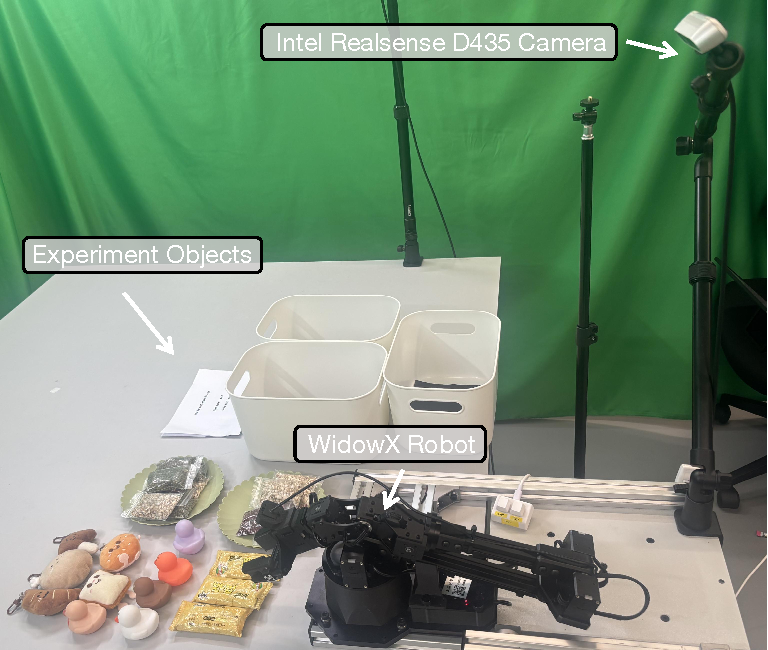
\includegraphics[width=0.9\linewidth]{imgs/setting.pdf}
    \caption{Real-world experimental setup. The system consists of a WidowX-250 robot arm, a front-facing Intel RealSense D435 camera, and a tabletop workspace containing task objects and storage boxes.}
    \label{fig:real_robot_setup}
\end{figure}

During data collection, both the external camera and the wrist camera record RGB observations at 25\,Hz. Each trajectory is synchronized with robot proprioceptive states, including end-effector pose, joint states, and gripper state. After collection, raw trajectories are processed through a standardized preprocessing pipeline. All images are resized to $224 \times 224$, and the trajectories are temporally subsampled to 10\,Hz. The processed demonstrations are then converted into the LeRobot format for downstream training.


\section{Analysis of Sentry's Working Memory and Termination Policy}


\begin{figure}[h]
    \centering
    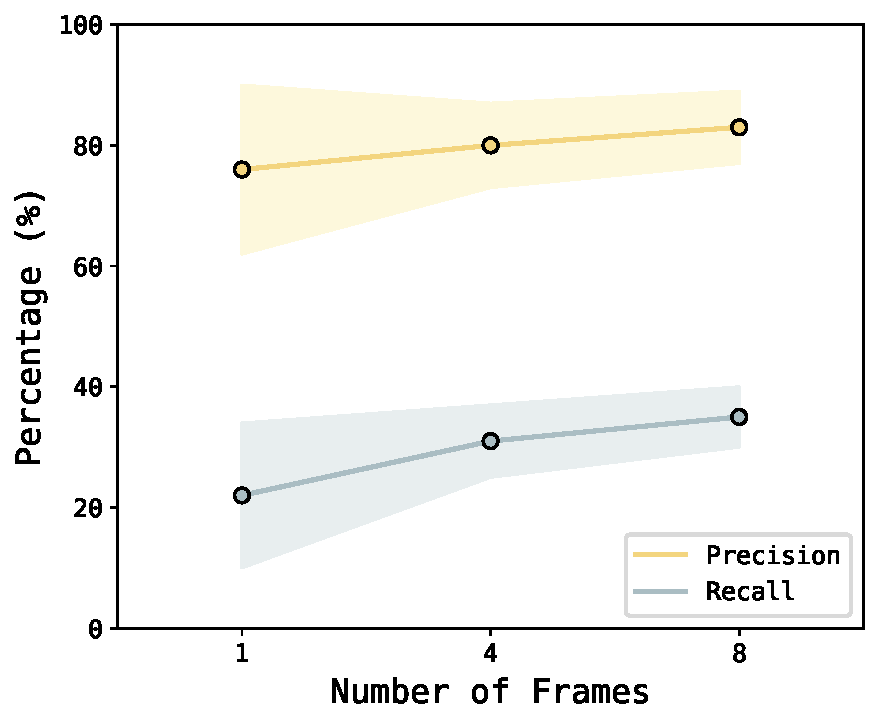
\includegraphics[width=.5\linewidth]{imgs/window_sentry.pdf}
    \caption{Increasing the number of recent frames provided to the Sentry leads to a consistent improvement in both precision and recall. This indicates that a longer temporal context is beneficial for accurate subtask monitoring.}
    \label{fig:sentry_ablation}
\end{figure}

To understand the Sentry's decision-making boundary, we analyzed its performance on subtask completion detection under different working memory sizes (window length $N$). \autoref{fig:sentry_ablation} presents the Precision and Recall, where Subtask ``Done'' is treated as the positive class.

% \siyin{standardize the scale and all use percentages.}
\textit{1) Benefits of Temporal Context:}
As shown in the \autoref{fig:sentry_ablation}, increasing the context window from 1 to 8 frames improves both Precision (from $\sim76\%$ to $\sim82\%$) and Recall (from $\sim22\%$ to $\sim35\%$).
A single frame often lacks sufficient information to distinguish between a temporary pause and true completion.
By observing a sequence of 8 frames (consistent with our sentry‘s working memory), the Sentry can leverage temporal cues to make more reliable judgments.

\textit{2) The "Conservative" Nature of Sentry:}
The significant gap between high Precision and low Recall reveals the Sentry's inherent ``conservative'' nature.
The system exhibits a strong bias towards the incomplete state, preferring to continue execution unless overwhelmingly confident that the goal is met.
While this minimizes premature stops (high Precision), the low Recall creates a ``missing signal'' problem where the agent might overshoot its target or enter infinite loops.
Since the Sentry is prone to False Negatives (missing the ``Done'' event), we design a fixed-interval Planner fallback.It ensures that execution loops are eventually broken even when the Sentry fails to trigger.

\section{Additional Experiments}
\label{sec:additional_experiments}

We provide additional experiments to further analyze controlled memory management, planner generalization with open-source VLMs, memory scalability over extended horizons, and system latency.

\subsection{Controlled Memory Ablation}
\label{sec:controlled_memory_ablation}

We first conduct a controlled memory ablation on the \textbf{Rearrangement} task to separate the effect of memory management strategy from that of memory capacity. In the main setting, HiMe uses unconstrained active memory, while the FIFO baseline is evaluated with a fixed memory budget. Although the FIFO budget is chosen to match the average memory size of the unlimited active baseline, the two settings still differ in whether memory is explicitly constrained. To provide a cleaner comparison, we additionally evaluate a limited-memory version of active management under the same fixed budget.

Specifically, we compare three variants: \textbf{Unlimited Active Management}, corresponding to the original HiMe setting with unconstrained memory; \textbf{Limited Active Management}, which uses the same Add / Update / Delete mechanism under a fixed budget of 8 entries; and \textbf{FIFO (Limited)}, which uses the same budget with FIFO eviction.

\begin{table}[H]
\centering
\caption{Controlled memory in Rearrangement.}
\label{tab:controlled_memory_ablation}
\begin{tabular}{lcc}
\toprule
\textbf{Method} & \textbf{Memory Budget} & \textbf{Task Progress (\%)} \\
\midrule
Unlimited Active Management & Unbounded & 87.0 \\
Limited Active Management & Fixed (8 entries) & 80.0 \\
FIFO (Limited) & Fixed (8 entries) & 64.0 \\
\bottomrule
\end{tabular}
\end{table}

Performance decreases under constrained memory, but active management remains substantially stronger than FIFO under the same capacity. This result indicates that the benefit of HiMe is not explained by larger memory alone, and that explicit Update / Delete operations remain useful beyond simple eviction.

\subsection{Open-Source Planner Evaluation}
\label{sec:opensource_planner_eval}

To improve reproducibility and examine planner generalization, we replace the main Planner with the open-source VLM \textbf{Qwen3-VL-30B} and evaluate the system on the \textbf{Rearrangement} task under the same protocol. The results are shown in Fig.~\ref{fig:qwen_appendix_more_exp}.

Fig.~\ref{fig:qwen_appendix_more_exp}(a) reports the main comparison with the corresponding baselines. Fig.~\ref{fig:qwen_appendix_more_exp}(b) presents the modality ablation, comparing the full system with text-only and image-only memory. Fig.~\ref{fig:qwen_appendix_more_exp}(c) shows the memory ablation under the same open-source Planner. Overall, the trends are consistent with the main experiments: HiMe remains the best-performing variant with Qwen3-VL-30B, indicating that the benefits of structured memory and sentry-based coordination are robust to the choice of Planner.

\begin{figure}[H]
    \centering
    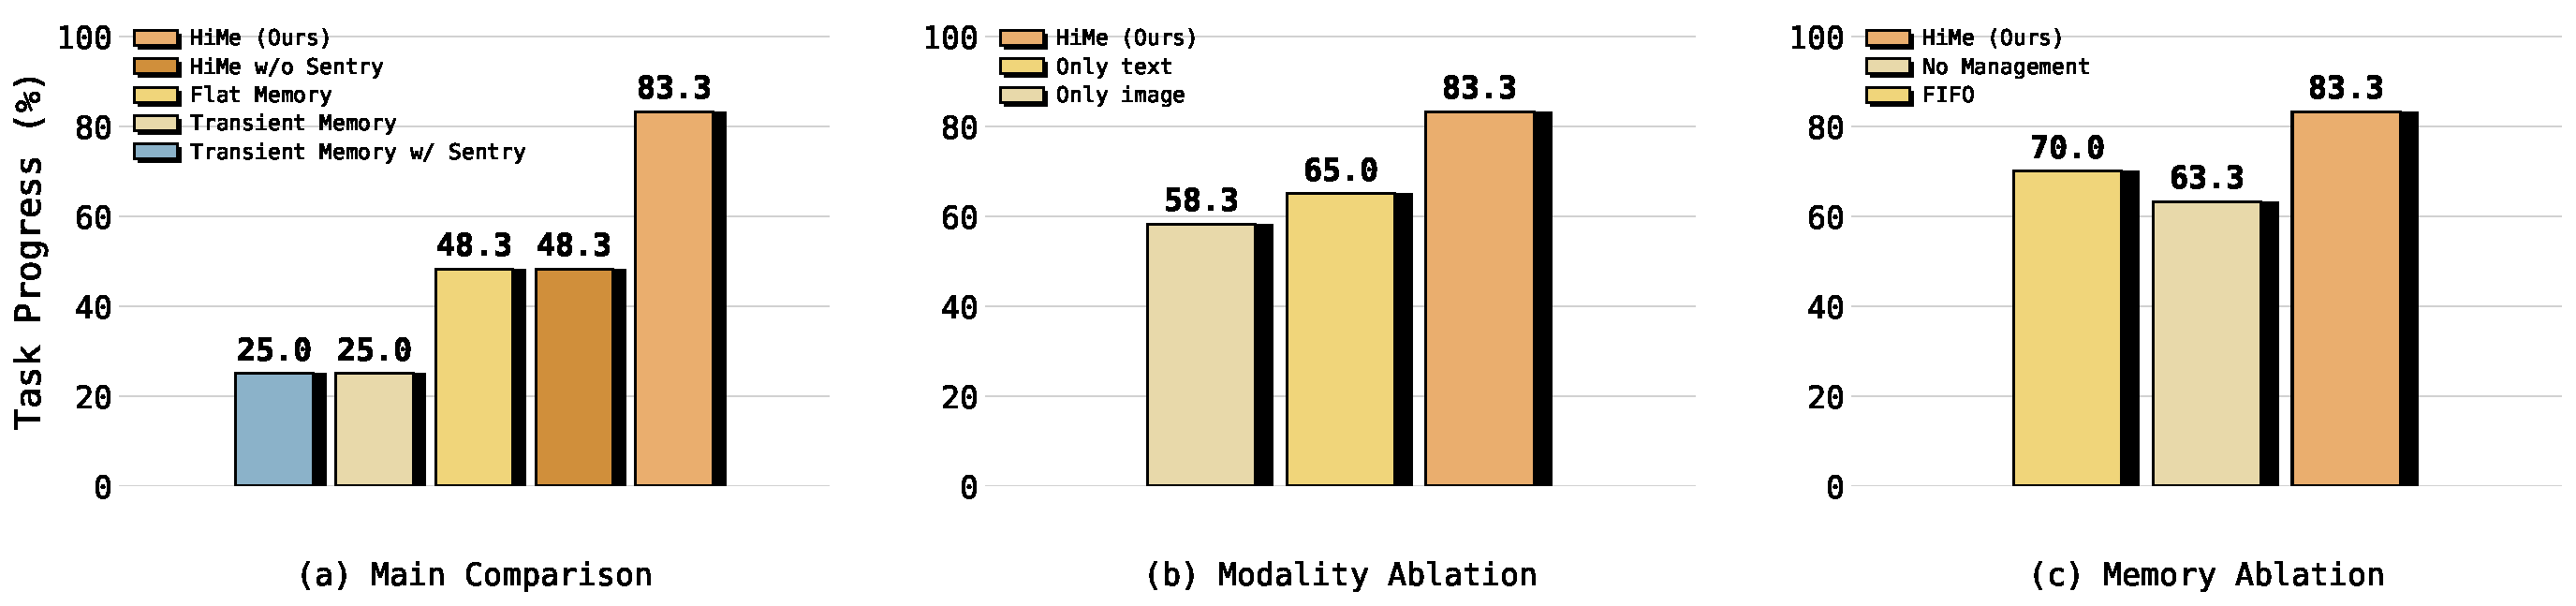
\includegraphics[width=\linewidth]{imgs/appendix_more_exp.pdf}
    \caption{Additional experiments on the \textbf{Rearrangement} task with \textbf{Qwen3-VL-30B} as the Planner. (a) Main comparison with the corresponding baselines. (b) Modality ablation. (c) Memory ablation. The overall trends are consistent with the main experiments, and HiMe remains the best-performing variant under the open-source Planner.}
    \label{fig:qwen_appendix_more_exp}
\end{figure}

\subsection{Memory Scalability}
\label{sec:memory_scalability}

We further analyze memory scalability using an extended multi-round version of \textbf{Object Search}. In each round, the robot must inspect boxes with initially unknown contents and place the visible table object accordingly. At the beginning of each new round, the box contents are changed, requiring the agent to re-inspect the scene and revise memory before acting. As the number of rounds increases, both the task horizon and the number of subtasks increase.

We report the average \textbf{Memory Size} and \textbf{Task Progress} across different numbers of rounds.

\begin{table}[H]
\centering
\caption{Memory scalability in extended multi-round Object Search.}
\label{tab:memory_scalability}
\begin{tabular}{cccc}
\toprule
\textbf{Rounds} & \textbf{Subtasks} & \textbf{Memory Size} & \textbf{Task Progress (\%)} \\
\midrule
1 & 4  & 5.5  & 92.5 \\
2 & 8  & 9.9  & 76.3 \\
3 & 12 & 14.0 & 66.7 \\
\bottomrule
\end{tabular}
\end{table}

As the horizon increases, memory size grows while task performance declines. This result suggests that the main challenge in long-horizon settings is not only storing more information, but also maintaining correct and up-to-date memory as the environment evolves.

\subsection{System Latency}
\label{sec:system_latency}

We additionally measure Planner latency under different deployments. Each Planner call consists of two stages: memory query / retrieval, and plan generation together with memory update. We report end-to-end latency over complete Planner calls.

\begin{table}[H]
\centering
\caption{End-to-end Planner latency under different model deployments.}
\label{tab:system_latency}
\begin{tabular}{lcccc}
\toprule
\textbf{Model} & \textbf{P50 (s)} & \textbf{P90 (s)} & \textbf{P99 (s)} & \textbf{Avg. Completion Tokens} \\
\midrule
GPT-4o (API) & 38.59 & 49.30 & 57.28 & 517.9 \\
Qwen3-VL-30B (local) & 6.83 & 7.93 & 8.65 & 532.8 \\
Qwen3-VL-8B (local) & 6.10 & 7.08 & 11.34 & 399.0 \\
\bottomrule
\end{tabular}
\end{table}

Latency differences are mainly associated with deployment mode, i.e., remote API versus local serving, rather than token scale alone. In practice, HiMe is compatible with different planner backends, and local deployment substantially reduces reasoning latency. Since Planner calls are triggered only when necessary, this reasoning latency remains decoupled from the high-frequency low-level control loop.

\newpage
\section{Prompts Details}

\begin{tcolorbox}[colback=black!2, colframe=black!45, title=Sentry Prompt]
You are the \textbf{EXECUTION OBSERVER} of an embodied agent.

\textbf{Primary input modality:}
\begin{itemize}[leftmargin=*]
    \item \textbf{Plan list:}
    \begin{itemize}
        \item The model’s current decomposition of the task into subtasks.
        \item Each subtask line includes its execution status (e.g., [done], [current], [pending]).
    \end{itemize}
    
    \item \textbf{Combined images of recent frames:}
    \begin{itemize}
        \item \textbf{CRITICAL LAYOUT INFO:} Each image is a composite.
        \item LEFT HALF: Wrist Camera View (Close-up, attached to the gripper).
        \item RIGHT HALF: Third-Person View (Global view of the robot and environment).
    \end{itemize}
\end{itemize}

Your \textbf{ONLY} job is to judge whether the \textbf{CURRENT} subtask has been completed.

\textbf{Judgment Criteria:}
\begin{itemize}[leftmargin=*]
    \item \textbf{Inspect:} done when the robot arm is above or extended into the box, and the wrist view shows the content and the black background of the box.
    
    \item \textbf{Pick \& Place:} done when the object has been successfully released at the destination or you observe that the robot arm is above a box and see its black background.
    
    \item \textbf{Reset:} done when the robot arm is in the home pose.
    \begin{itemize}
        \item The robot arm home pose is: in both images, the arm is aligned parallel to what appears to be a rail or track. The end effector (or gripper) is open and facing downwards towards the table.
    \end{itemize}
    
    \item The interior bottom surface of the box is lined with a black background to enhance contrast for detection.
\end{itemize}

\noindent\rule{\linewidth}{0.4pt} % 分割线

\textbf{\# REQUIRED OUTPUT FORMAT}

You \textbf{MUST} output exactly this XML structure:

\begin{verbatim}
<status>
<!-- EXACTLY one of:
        done
        not_done
-->
</status>
\end{verbatim}

\end{tcolorbox}

\begin{tcolorbox}[
    enhanced,                   % 启用增强绘图引擎（修复渲染问题）
    colback=white,              % 强制背景为纯白 (如果觉得太亮，可改为 black!5)
    colframe=blue!50!black,     % 边框颜色：深蓝
    coltext=black,              % 强制文字为黑色
    title=Planner Prompt,
    fonttitle=\bfseries,        % 标题加粗
    breakable,                  % 允许跨页
    arc=2mm                     % 圆角大小
]

You are the \textbf{PLANNER} of an embodied agent.

\textbf{Primary input modalities:}
\begin{itemize}[leftmargin=*]
    \item \textbf{User instruction:} The user's high-level instruction for the agent.
    \item \textbf{Plan list:} The model's current decomposition of the task into subtasks. Each subtask line includes its execution status (e.g., [done], [current], [pending]).
    \item \textbf{Combined images during subtask execution:}
    \begin{itemize}
        \item \textbf{IMAGE LAYOUT \& USAGE GUIDE:}
        \item \textbf{LEFT HALF (Wrist View):} Egocentric view attached to the gripper. Usage: Identify specific objects, read text, verify grasping.
        \item \textbf{RIGHT HALF (Third-Person View):} Global view. Usage: Spatial context, locating containers, tracking arm position.
        \item \textbf{NOTE:} Integrate information from both. Use Right view to navigate, Left view to inspect.
    \end{itemize}
\end{itemize}

You have access to an external \textbf{MEMORY} module through a structured CRUD interface.
MEMORY stores records with fields: \texttt{id}, \texttt{tags}, \texttt{data} (type, value), \texttt{image\_path}.

\noindent\rule{\linewidth}{0.4pt}

\textbf{\# TAG DESIGN PRINCIPLES}

Tags are the PRIMARY mechanism for memory retrieval.

\begin{enumerate}[leftmargin=*]
    \item \textbf{OBJECT TAGS:} \texttt{toy\_duck}, \texttt{snack\_package}, \texttt{left\_box}.
    \item \textbf{LOCATION TAGS:} \texttt{table}, \texttt{shelf}, \texttt{inside\_left\_box}.
    \item \textbf{USER\_PREFERENCE TAGS:} \texttt{user}, \texttt{lily}, \texttt{likes}, \texttt{prefers}.
\end{enumerate}

\textbf{Tag Usage Rules:} Use 2-5 tags per record. Update tags when object state changes.
\textbf{Tag Query Strategy:} PREFER tag-based queries. Query one tag every time.

\noindent\rule{\linewidth}{0.4pt}

\textbf{\# MEMORY CRUD PROTOCOL}

You interact with memory only via structured XML operations.

\textbf{(1) QUERY (READ)}
\begin{verbatim}
<operation>
  <type>QUERY</type>
  <query>search key tags</query>
  <reason>why you search this</reason>
</operation>
\end{verbatim}

\textbf{(2) CREATE}
\begin{verbatim}
<operation>
  <type>CREATE</type>
  <tags>...</tags>
  <text>concise description or fact</text>
  <image_path>index</image_path>
  <reason>why this new memory is necessary</reason>
</operation>
\end{verbatim}

\textbf{(3) UPDATE}
\begin{verbatim}
<operation>
  <type>UPDATE</type>
  <id>record_id</id>
  <tags>...</tags>
  <text>updated description</text>
  <image_path>2</image_path>
  <reason>why this existing record must be changed</reason>
</operation>
\end{verbatim}

\textbf{(4) DELETE}
\begin{verbatim}
<operation>
  <type>DELETE</type>
  <id>...</id>
  <reason>why this record is no longer useful</reason>
</operation>
\end{verbatim}

\noindent\rule{\linewidth}{0.4pt}

\textbf{\# EVIDENCE RELIABILITY RULES (NO ASSUMPTIONS)}
\begin{itemize}[leftmargin=*]
    \item Memory must contain only verifiable facts derived from explicit user instructions or direct visual evidence.
    \item \textbf{Do NOT CREATE FAKE memory.} Prefer planning an inspection step.
    \item UPDATE is for correcting/refining without changing time meaning.
    \item When state changes, \textbf{CREATE} a new record, UPDATE the old one to label as past.
    \item DELETE sparingly (only for duplicates or errors).
\end{itemize}

\noindent\rule{\linewidth}{0.4pt}

\textbf{\# MEMORY USAGE POLICY (TWO-TURN INTERACTION)}
\begin{itemize}[leftmargin=*]
    \item \textbf{Turn 1 (QUERY-only):} Issue QUERY operations. NO Create/Update/Delete. Plan list must be empty.
    \item \textbf{Turn 2 (REFINE + CRUD):} Issue Create/Update/Delete based on query results. Output finalized \texttt{<plan\_list>}.
\end{itemize}

\noindent\rule{\linewidth}{0.4pt}

\textbf{\# PLAN LIST FORMAT (FINAL OUTPUT ONLY, TURN 2)}
Plain text, one subtask per line.
\begin{itemize}
    \item \texttt{[done]}: subtask completed.
    \item \texttt{[current]}: the single subtask to execute NEXT.
    \item \texttt{[pending]}: future subtasks.
\end{itemize}
Annotation: You MAY include a short purpose in parentheses, e.g., \texttt{[pending] inspect recipe (check what does it need)}.

\noindent\rule{\linewidth}{0.4pt}

\textbf{\# PLAN LIST ACTION FORMAT}
\begin{enumerate}[leftmargin=*]
    \item \textbf{Inspection action:} Main verb "inspect". Use when information is missing.
    \item \textbf{Pick-and-place action:} "pick up \texttt{<object>} \texttt{<source>} and place it to \texttt{<target>}".
\end{enumerate}

\noindent\rule{\linewidth}{0.4pt}

\textbf{\# REQUIRED OUTPUT FORMAT FOR EACH TURN}

\begin{verbatim}
<summary>
  <!-- Concise reasoning summarizing observations and memory interaction -->
</summary>

<memory_operations>
  <!-- Turn 1: QUERY only. Turn 2: CRUD operations. -->
</memory_operations>

<plan_list>
  <!-- Turn 1: EMPTY.
       Turn 2: Finalized plan list.
       [done] ...
       [current] ...
       [pending] ...
  -->
</plan_list>
\end{verbatim}

\end{tcolorbox}





% \section{Case Study}
% memory content






%%%%%%%%%%%%%%%%%%%%%%%%%%%%%%%%%%%%%%%%%%%%%%%%%%%%%%%%%%%%%%%%%%%%%%%%%%%%%%%
%%%%%%%%%%%%%%%%%%%%%%%%%%%%%%%%%%%%%%%%%%%%%%%%%%%%%%%%%%%%%%%%%%%%%%%%%%%%%%%

\end{document}

% This document was modified from the file originally made available by
% Pat Langley and Andrea Danyluk for ICML-2K. This version was created
% by Iain Murray in 2018, and modified by Alexandre Bouchard in
% 2019 and 2021 and by Csaba Szepesvari, Gang Niu and Sivan Sabato in 2022.
% Modified again in 2023 and 2024 by Sivan Sabato and Jonathan Scarlett.
% Previous contributors include Dan Roy, Lise Getoor and Tobias
% Scheffer, which was slightly modified from the 2010 version by
% Thorsten Joachims & Johannes Fuernkranz, slightly modified from the
% 2009 version by Kiri Wagstaff and Sam Roweis's 2008 version, which is
% slightly modified from Prasad Tadepalli's 2007 version which is a
% lightly changed version of the previous year's version by Andrew
% Moore, which was in turn edited from those of Kristian Kersting and
% Codrina Lauth. Alex Smola contributed to the algorithmic style files.
